\documentclass[aspectratio=169]{beamer}
\usepackage{will_handley_beamer}
\usepackage{title_page}
\usepackage{listings}
\usepackage{xcolor}

\definecolor{codegreen}{rgb}{0,0.6,0}
\definecolor{codegray}{rgb}{0.5,0.5,0.5}
\definecolor{codepurple}{rgb}{0.58,0,0.82}
\definecolor{backcolour}{rgb}{0.95,0.95,0.92}

\lstdefinestyle{mystyle}{
    backgroundcolor=\color{white},   
    commentstyle=\color{C2},
    keywordstyle=\color{C3},
    numberstyle=\tiny\color{C0},
    stringstyle=\color{C1},
    basicstyle=\ttfamily\tiny,
	identifierstyle=\color{black},
    breakatwhitespace=false,         
    breaklines=true,                 
    captionpos=b,                    
    keepspaces=true,                 
    numbers=left,                    
    numbersep=5pt,                  
    showspaces=false,                
    showstringspaces=false,
    showtabs=false,                  
    tabsize=2
}

\lstset{style=mystyle}


% Commands
% --------
% - \arxiv{arxiv number}
% -  \begin{fig(left|right)}[fractional width (e.g 0.6) ]{name of image}
%        content of other column
%    \end{fig(left|right)}

% Talk details
% ------------
\title{Sampling techniques in high-dimensional parameter spaces}
\subtitle{with ScannerBit 2.0}
\date{23\textsuperscript{rd} Feb 2024}

\begin{document}

\begin{frame}
    \titlepage
\end{frame}

\begin{frame}
    \frametitle{What do I mean by parameter spaces?}
    \begin{itemize}
        \item In science we build models $M$ to describe data $D$
        \item These models usually come with a vector of tunable unknown parameters $\theta$
        \item The general task of science is to use data to define regions of ``good'' $\theta$
        \item This talks considers the (increasingly common) case where $\theta$ is high-dimensional
            \begin{itemize}
                \item High-dimensional: $d\ge4$
            \end{itemize}
        \item Let's look at some concrete examples across fields
    \end{itemize}
\end{frame}

\begin{frame}
    \frametitle{Cosmology \& Astrophysics}
    \begin{columns}
        \column{0.4\textwidth}
        \begin{itemize}
            \item Cosmological parameters:%
                \begin{itemize}
                    \item matter fraction $\Omega_m$
                    \item dark matter $\Omega_b$
                    \item dark energy $\Omega_\Lambda$
                    \item Hubble constant $H_0$
                    \item Initial conditions $(A_s, n_s)$
                    \item optical depth $\tau$
                \end{itemize}
            \item LIGO/Virgo/Kagra event:%
                \begin{itemize}
                    \item masses $m_1, m_2$
                    \item spins $\chi_1, \chi_2$
                    \item sky position $(\theta, \phi)$
                    \item orientation $(\iota, \psi)$
                    \item distance $d_L$
                    \item time \& phase $t_c, \Phi_c$
                \end{itemize}
            \item Bayesian framework: $P(\theta|D)$ defines ``credible regions''
        \end{itemize}
        
        \column{0.35\textwidth}
        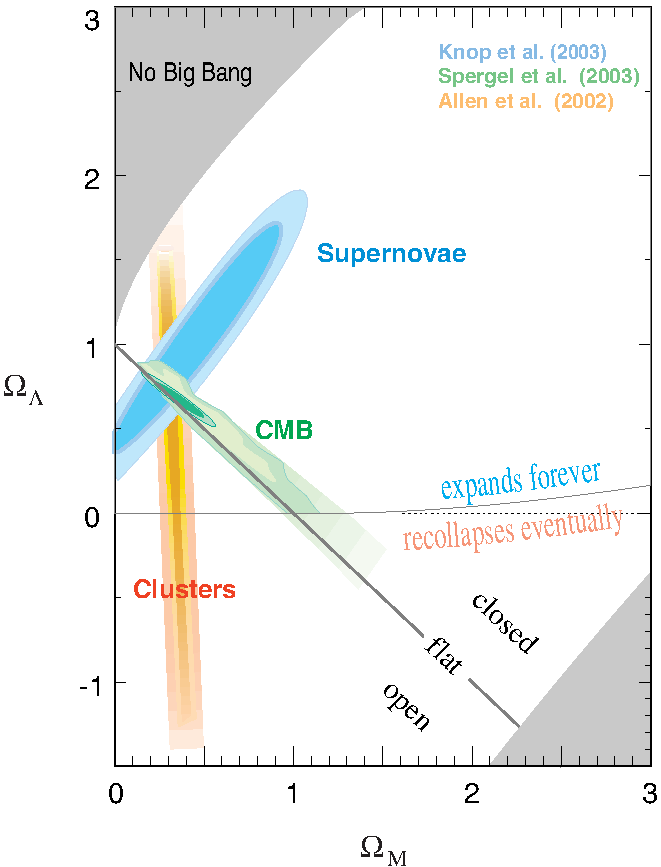
\includegraphics[width=\textwidth]{figures/old_parameters}
        \column{0.25\textwidth}
        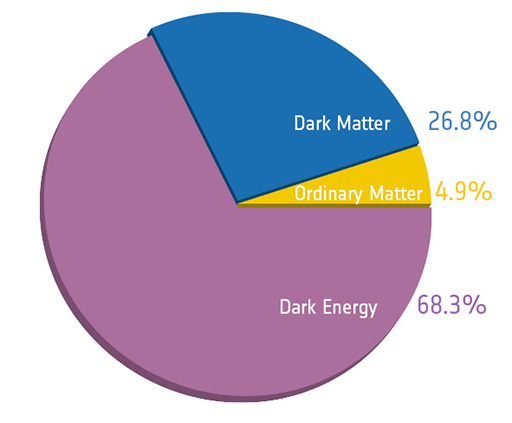
\includegraphics[width=\textwidth]{figures/darkmatterchart_squared}
        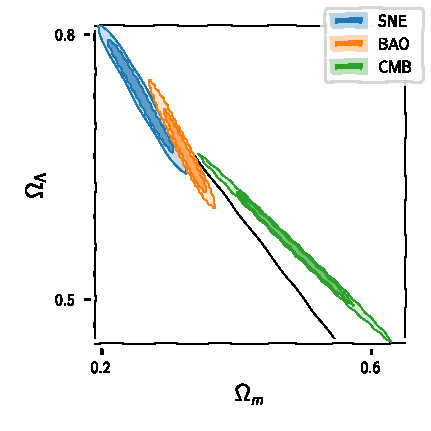
\includegraphics[width=\textwidth]{figures/universe_constraints_zoom}
        %TODO put in LIGO event
    \end{columns}

    
\end{frame}

\begin{frame}
    \frametitle{Particle physics}
    \begin{columns}
        \column{0.5\textwidth}
        \begin{itemize}
            \item The standard model has a several physical/phenomenological parameters
            \item Frequentist framework: $P(D|\theta)$ defines ``confidence intervals''
            \item topical: pMSSM ATLAS scans $d=19$
        \end{itemize}
        \centerline{
            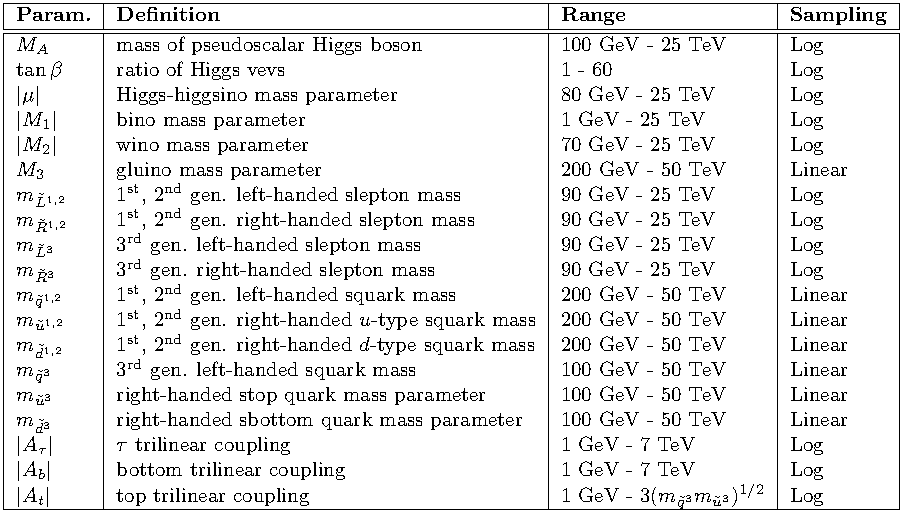
\includegraphics[width=\textwidth]{figures/pmssm}
        }
        \column{0.5\textwidth}
        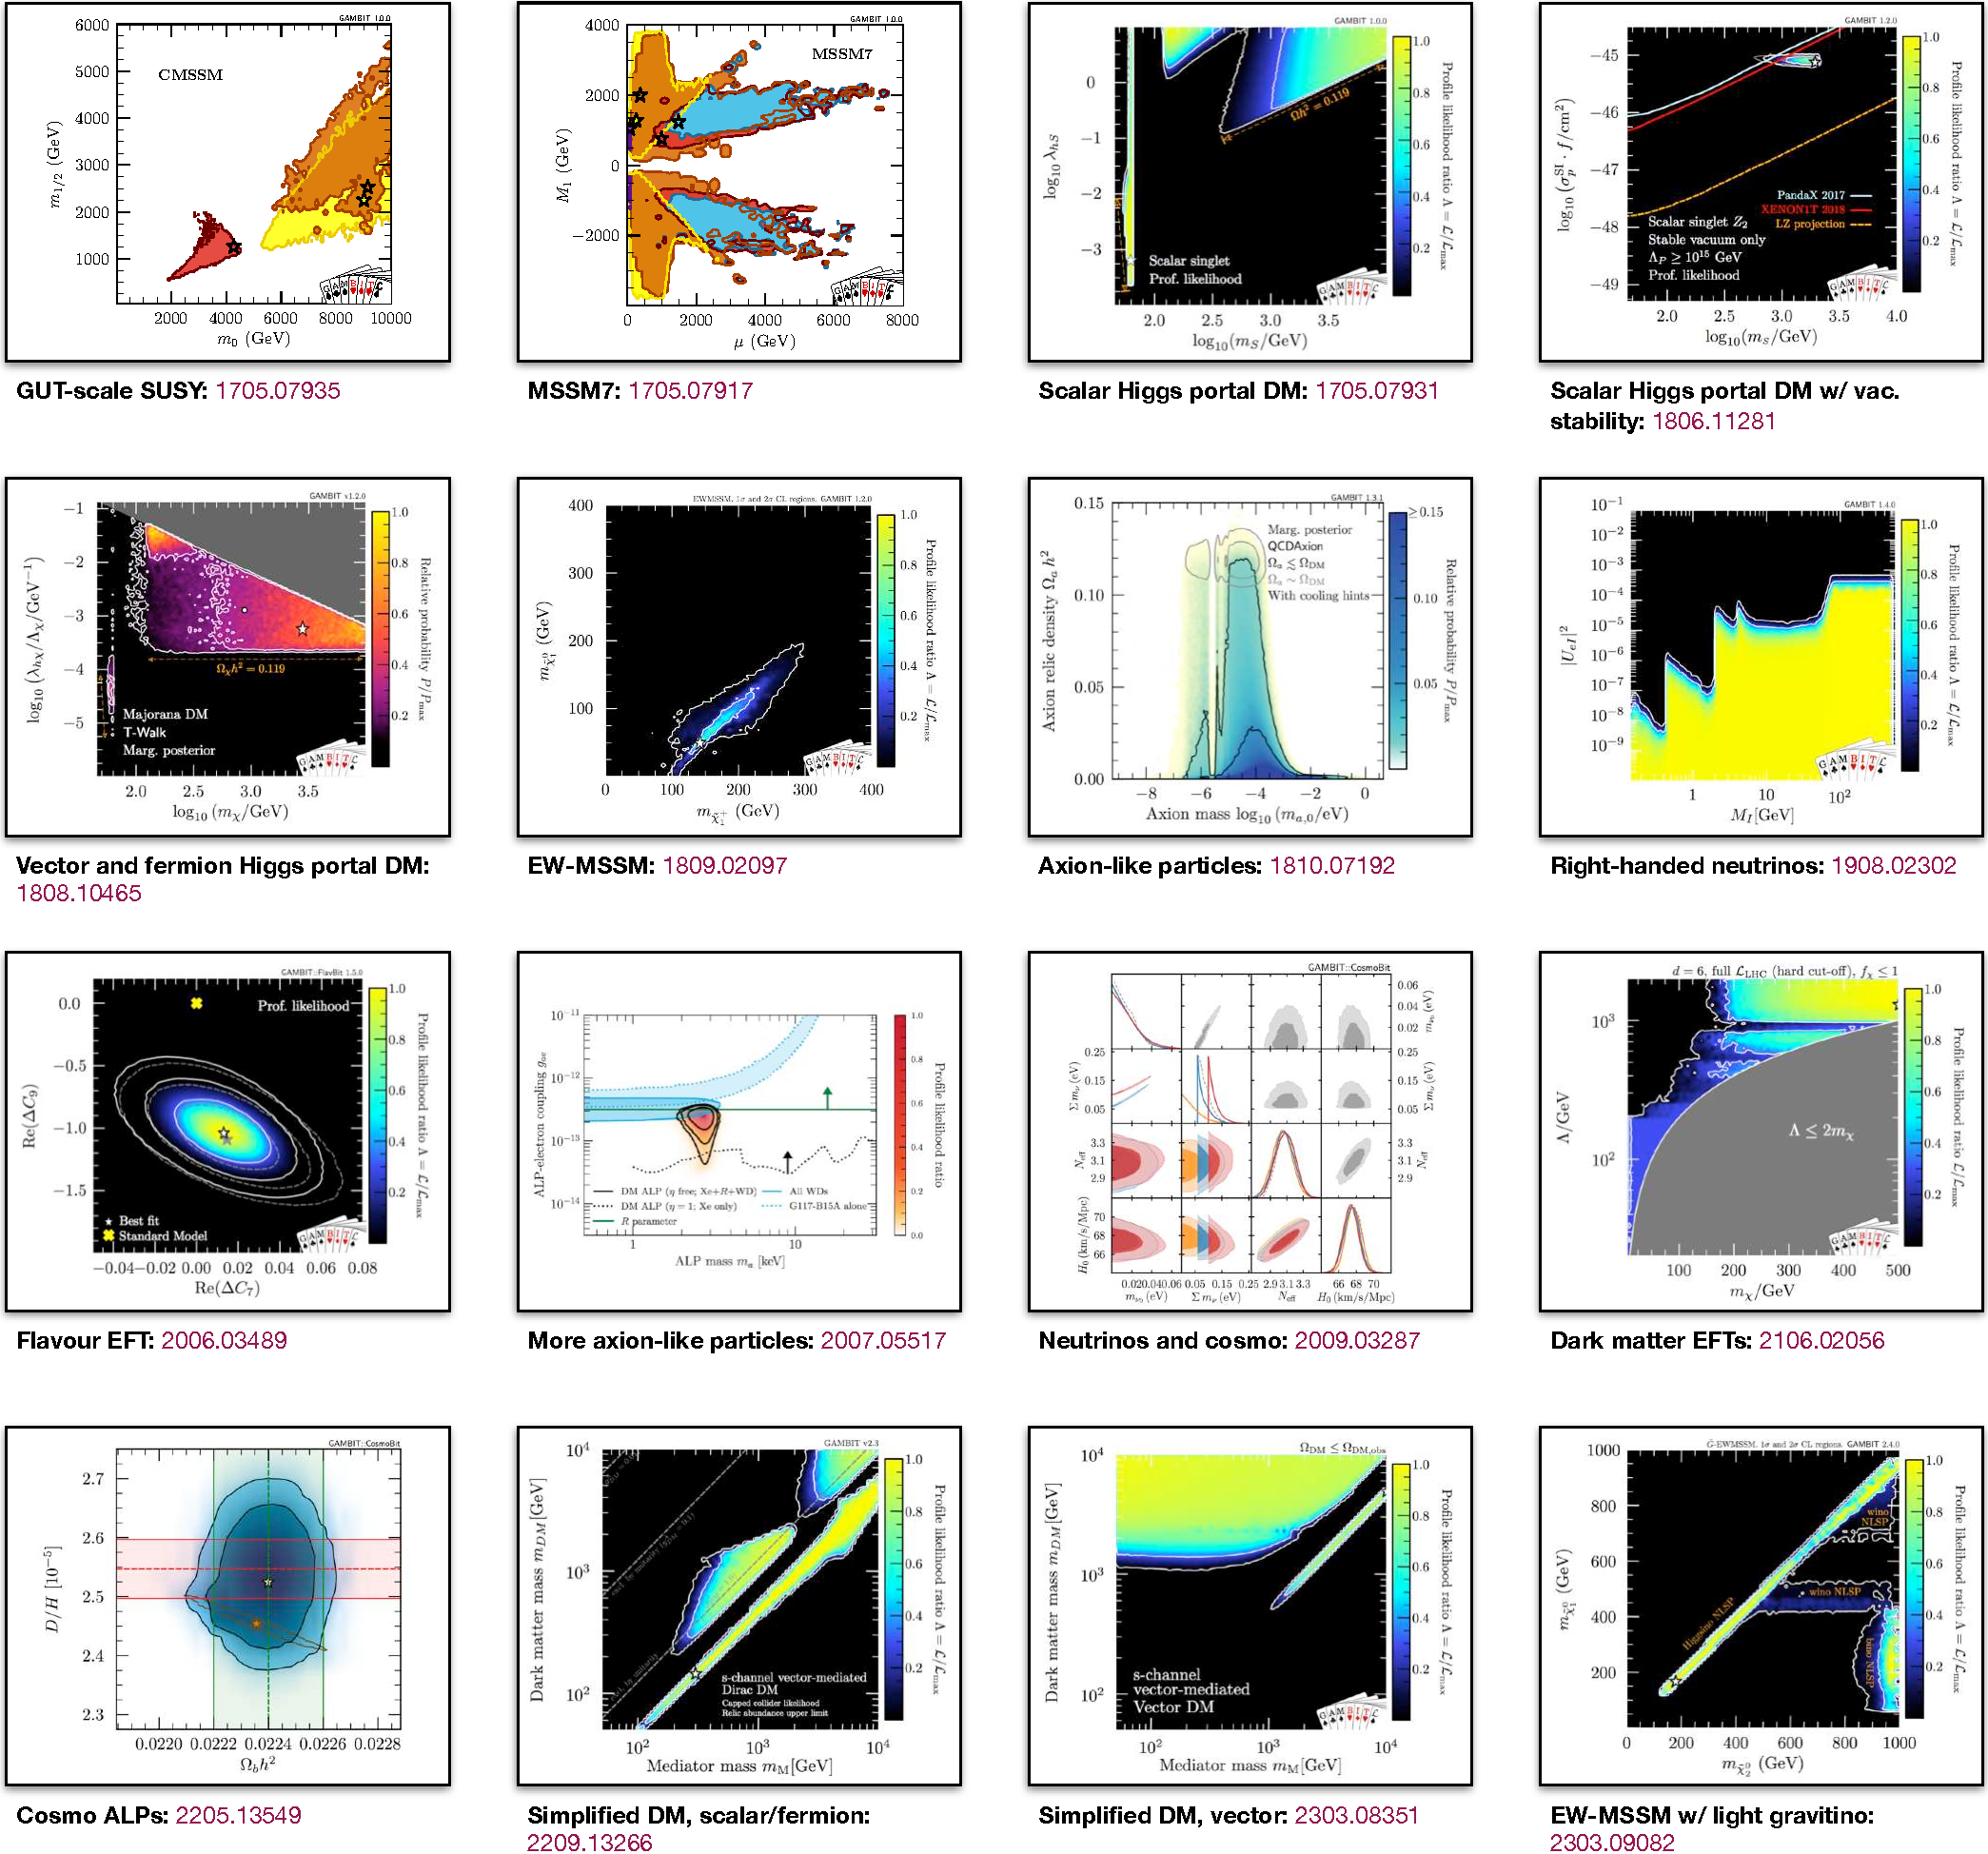
\includegraphics[width=\textwidth]{figures/gambit_examples}
    \end{columns}
    
\end{frame}

\begin{frame}
    \frametitle{Materials/Chemistry}
    \begin{columns}
        \column{0.65\textwidth}
        \begin{itemize}
            \item Here the relevant function is the free energy $F(\theta)$ as a function of system configuration (bond angles, bond lengths).
            \item Naturally very high dimensional $d\sim\mathcal{O}(10^2\to10^5)$.
            \item Complicated parameter spaces with many solutions of interest
            \item Boltzmann distribution $P(\theta) = e^{-\beta E(\theta)}$ defines the thermodnamic ensemble.
            \item Added challenge of temperature free parameter, meaning ideally one wants $Z(\beta) = e^{-\beta F(\beta)} = \int P(\theta|\beta) d\theta$
        \end{itemize}
        
        \column{0.35\textwidth}
        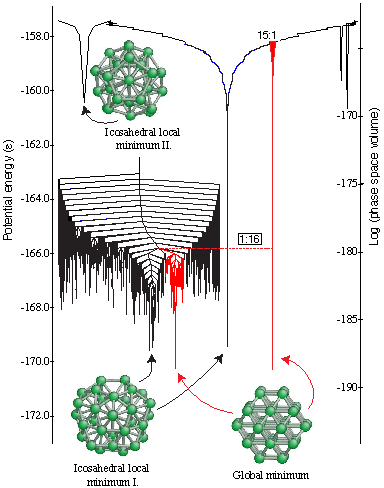
\includegraphics[width=\textwidth]{figures/materials}
        
    \end{columns}
\end{frame}

\begin{frame}
    \frametitle{Biophysics}
    \begin{columns}
        \column{0.5\textwidth}
        \begin{itemize}
            \item Specific example is protein molecules
            \item Alphafold made waves in this space in 2022
            \item Essentially a powerful machine learning optimisation solution
            \item Full problem is far from solved!
            \item Ideally one would compute misfolds \& partition functions
        \end{itemize}
        
        \column{0.5\textwidth}
        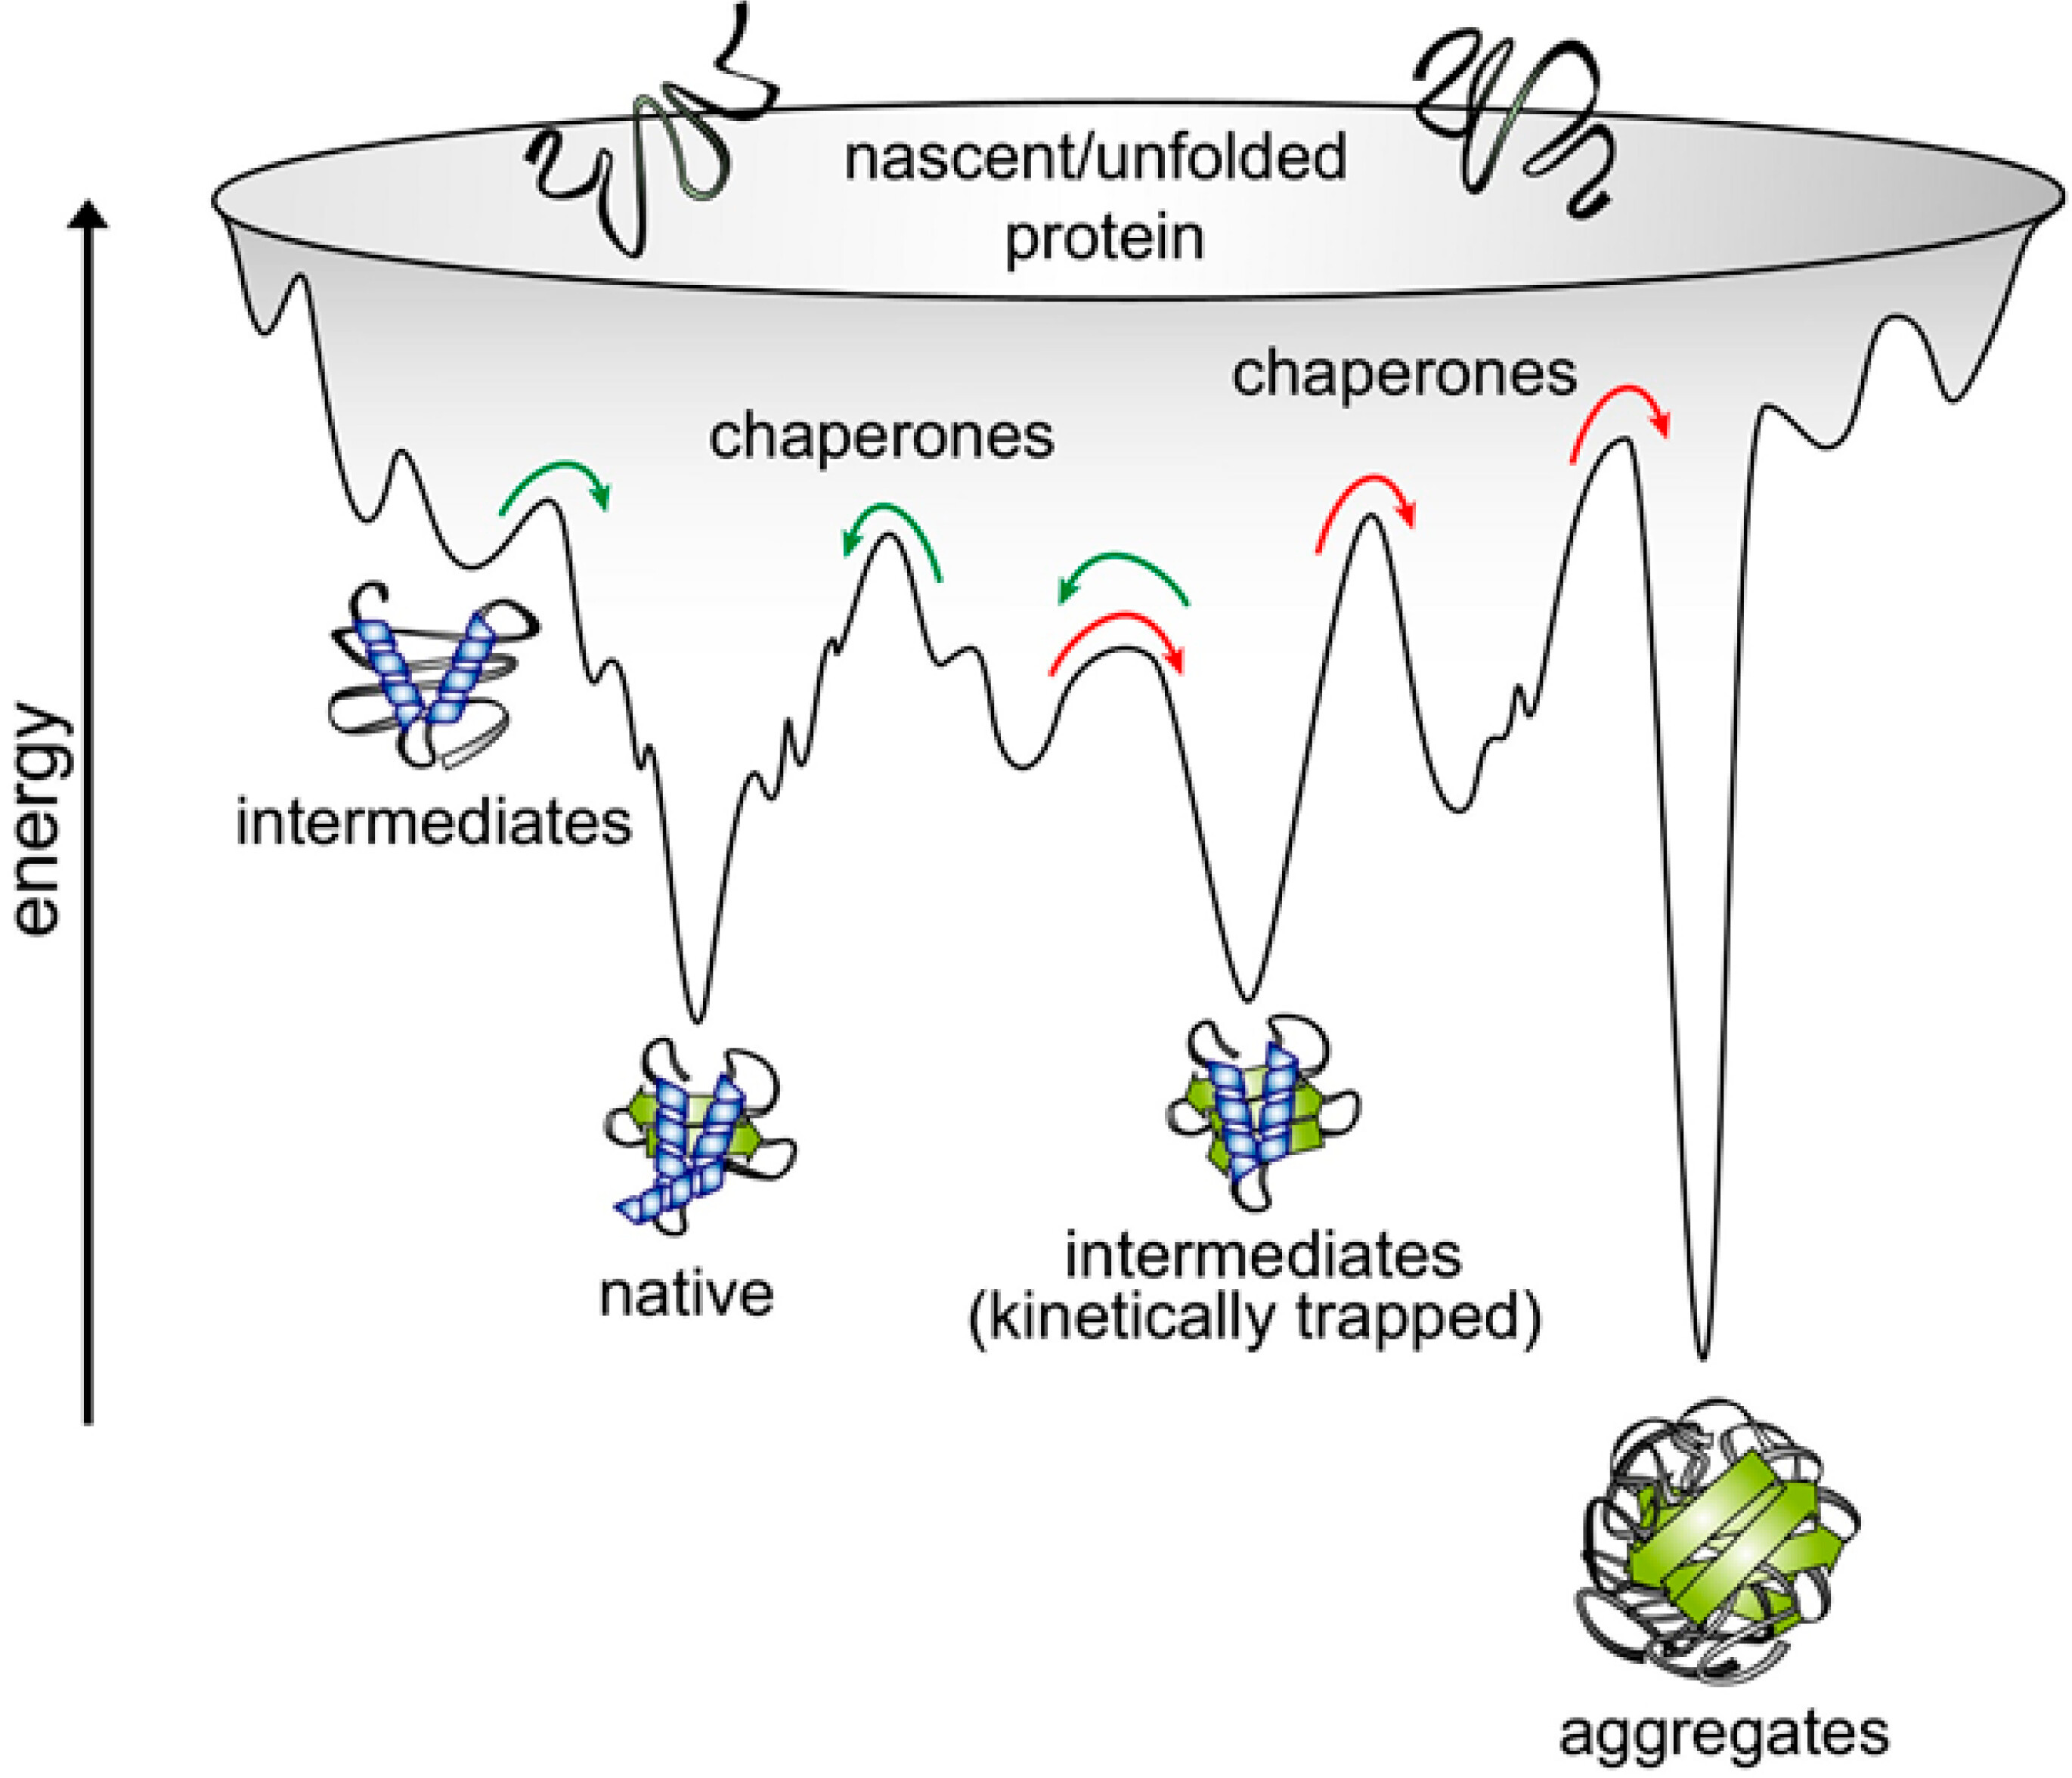
\includegraphics[width=\textwidth]{figures/proteins}
        
    \end{columns}
\end{frame}

\begin{frame}
    \frametitle{Machine learning}
    \begin{columns}
        \column{0.5\textwidth}
        \begin{itemize}
            \item Standard machine learning training setup:
                \[ \hat{\theta} = \min_\theta L(\theta) \]
                \[ L(\theta) = \min_{\theta} \sum_{i\in\text{train}} |f(x_i;\theta)-y_i|^2 \]
                \begin{itemize}
                    \item $x$: input data
                    \item $y$: target data
                    \item $f$: neural network
                    \item $\theta$: model parameters (weights and biases)
                \end{itemize}
            \item The ``Loss function'' $L$ of the training/testing data defines the ``good'' $\theta$
            \item Usually optimised with gradient descent (adam).
        \end{itemize}
        
        \column{0.5\textwidth}
        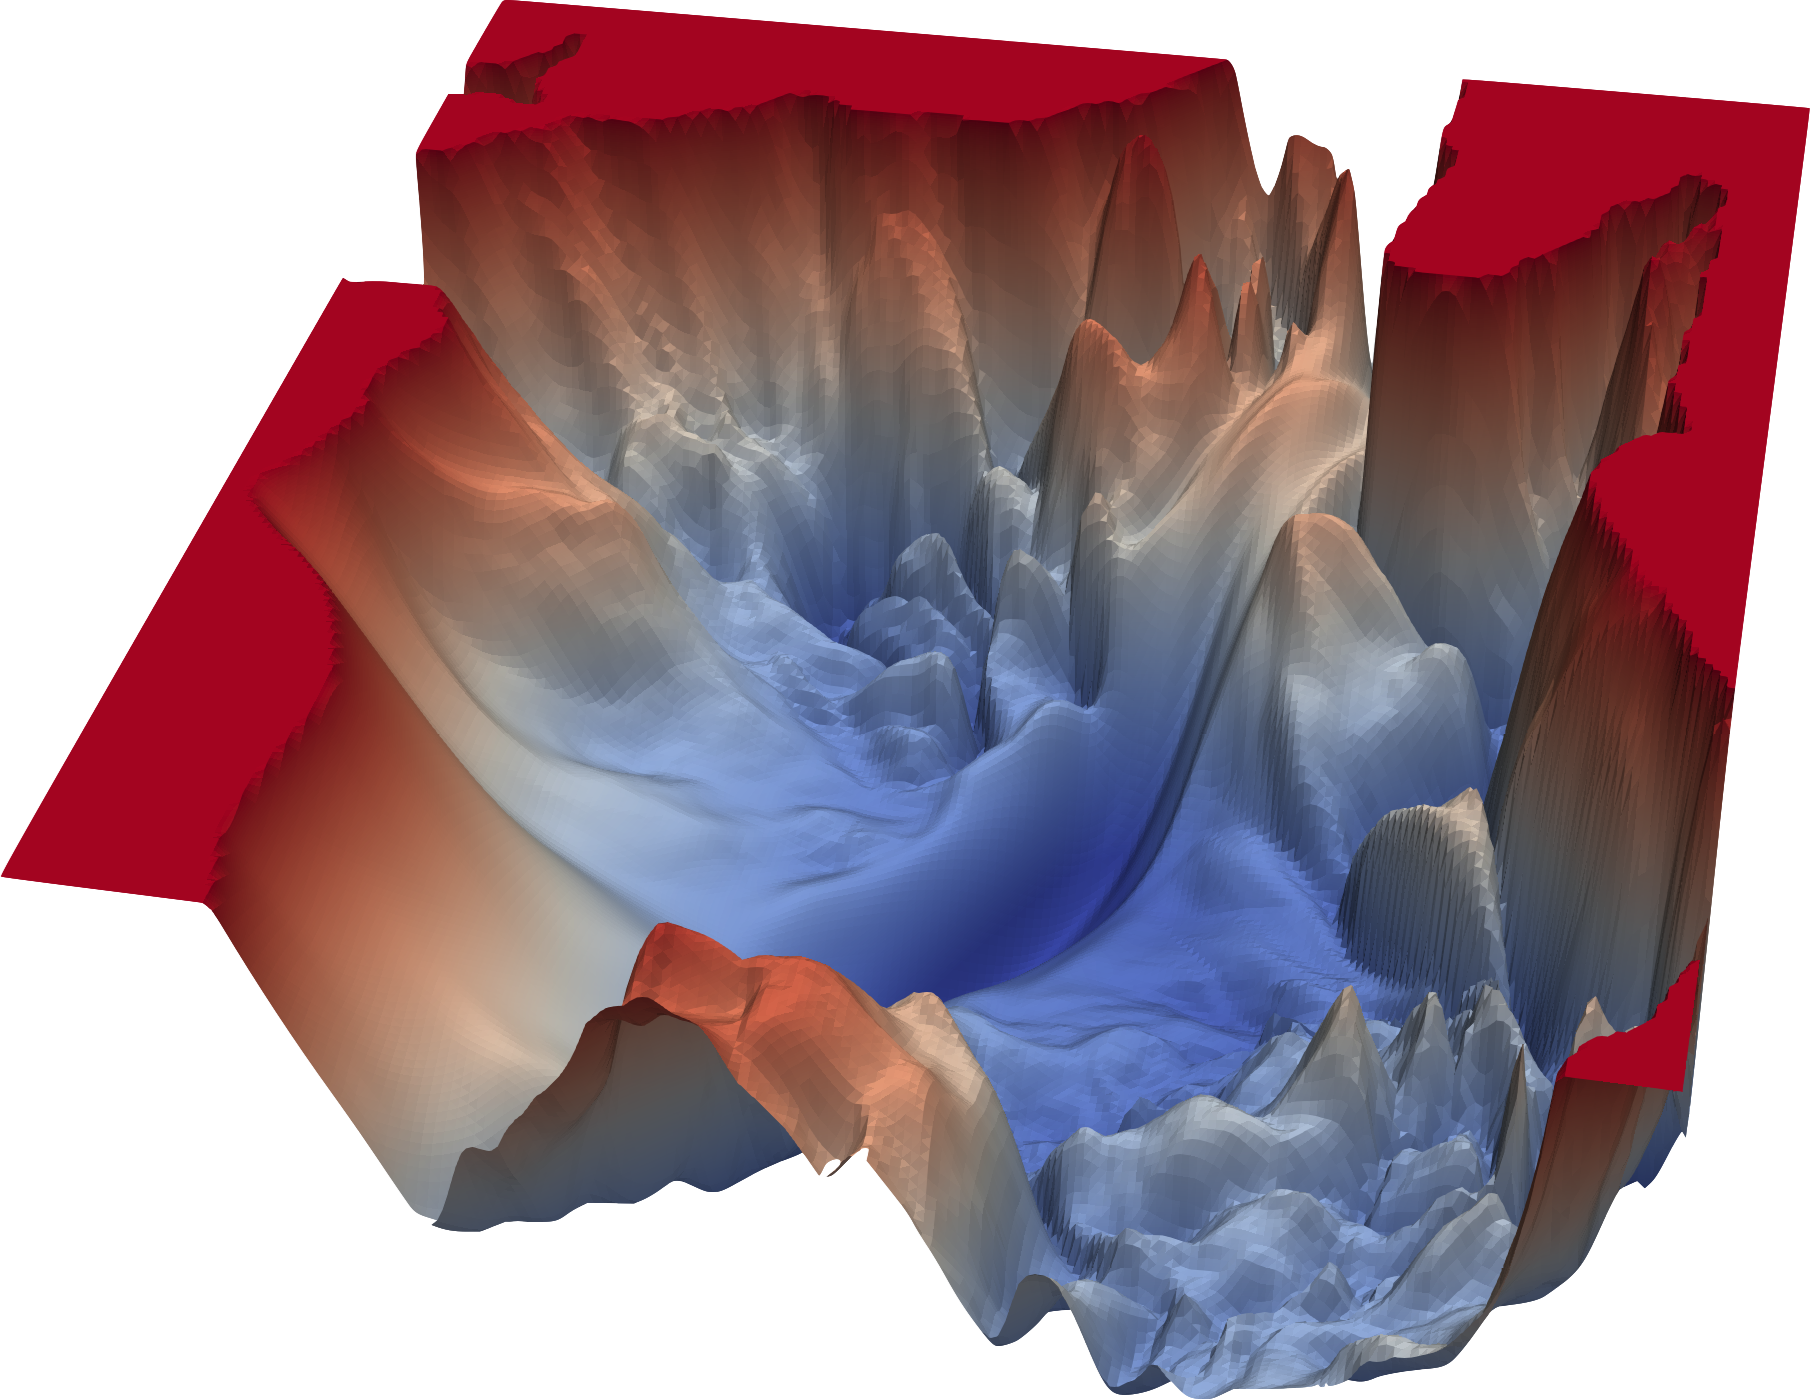
\includegraphics[width=\textwidth]{figures/loss_landscape}

        \hfill\href{https://losslandscape.com}{losslandscape.com}
    \end{columns}
\end{frame}

\begin{frame}[fragile]
    \frametitle{Why is high-dimensional $d\ge4$?}
    \begin{columns}
        \column{0.5\textwidth}
        \begin{itemize}
            \item 4D is where 
            \item The ``curse of dimensionality''
            \item We can see this effect if we consider trying to do a 1, 2, 3 \& 4D integral numerically

            \item Visualisation requires a 2D projection
            \item 2D has very specific properties which do not lend themselves well to intuiting the behaviour of the full parameter space
        \end{itemize}
        \column{0.5\textwidth}
    \begin{lstlisting}[language=Python]
import numpy as np
from scipy.integrate import nquad

def f(*x):
    x = np.array([*x])
    return np.exp(-(x**2).sum())

nquad(f, [[-5, 5]])     # 322  micro s
nquad(f, [[-5, 5]] * 2) # 33.4 ms
nquad(f, [[-5, 5]] * 3) # 3.4  s 
nquad(f, [[-5, 5]] * 4) # ...
    \end{lstlisting}
        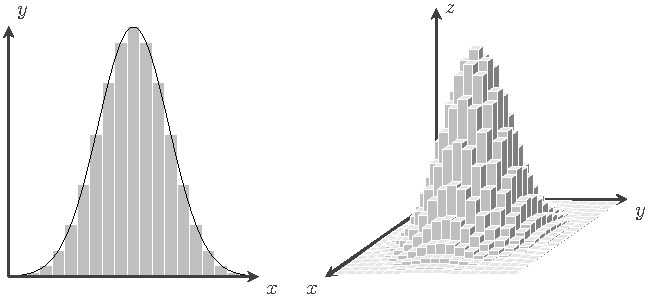
\includegraphics[width=\textwidth]{figures/integration.pdf}
    \end{columns}
    
\end{frame}

\begin{frame}
    \frametitle{Observation \#1: The typical set is small}

    \begin{columns}
        \column{0.6\textwidth}
    \begin{itemize}
        \item The non-zero region of the function (the typical set) occupies a tiny fraction of the space
        \item From a 1D/2D projected view, this is not obvious
        \item If each parameter has a compressed region $\delta\theta_i$ relative to the initial bounds $\Delta\theta_i$, then the total fraction of the compressed region is
            $\prod_i^d \frac{\delta \theta_i}{\Delta \theta_i}$
        which is exponential in the number of parameters $d$
    \item This is generalised by the KL divergence:
\[\mathcal{D}_\mathrm{KL} = \int \mathcal{P}(\theta) \log\frac{\mathcal{P}(\theta)}{\pi(\theta)} d\theta \sim \log \frac{V_\pi}{V_\mathcal{P}}\]
    \item e.g. $6d$ cosmological Planck $\Lambda$CDM $e^{-\mathcal{D}_\mathrm{KL}}\sim 10^{-14}$
    \end{itemize}
        
        \column{0.4\textwidth}
        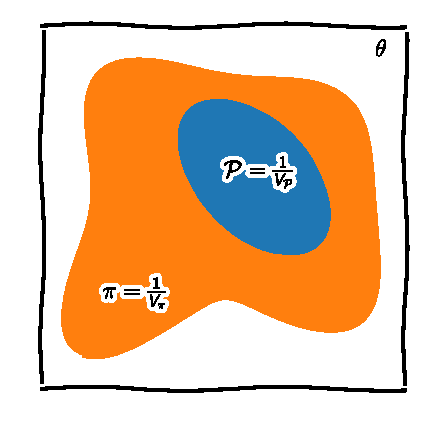
\includegraphics[width=\textwidth]{figures/volumes.pdf}
    \end{columns}

\end{frame}



\begin{frame}
    \frametitle{Observation \#2: The typical set is not at the peak}
    \begin{columns}
        \column{0.5\textwidth}
        \begin{itemize}
            \item In low dimensions, the ``best fit point'' is in the ``best fit region''.
            \item This is not true in high dimensions.
            \item This can be thought of as a balance of:
                \begin{itemize}
                    \item probability density and volume
                    \item energy and entropy
                    \item likelihood and prior
                \end{itemize}
        \end{itemize}
        
        \column{0.5\textwidth}
        \includegraphics<1>[width=\textwidth, page=1]{figures/anatomy}%
        \includegraphics<2>[width=\textwidth, page=2]{figures/anatomy}%
        \includegraphics<3>[width=\textwidth, page=3]{figures/anatomy}%
        \includegraphics<4>[width=\textwidth, page=4]{figures/anatomy}%
        \includegraphics<5>[width=\textwidth, page=5]{figures/anatomy}%
        \includegraphics<6>[width=\textwidth, page=6]{figures/anatomy}%
        \includegraphics<7>[width=\textwidth, page=7]{figures/anatomy}%
        \includegraphics<8>[width=\textwidth, page=8]{figures/anatomy}%
        \includegraphics<9>[width=\textwidth, page=9]{figures/anatomy}%
        \includegraphics<10>[width=\textwidth, page=10]{figures/anatomy}%
        \includegraphics<11>[width=\textwidth, page=11]{figures/anatomy}%
        \includegraphics<12>[width=\textwidth, page=12]{figures/anatomy}%
        \includegraphics<13>[width=\textwidth, page=13]{figures/anatomy}%
    \end{columns}
\end{frame}

\begin{frame}
    \frametitle{Principles of parameter exploration}
    \begin{enumerate}
        \item \textbf{What do I want to do?}  \textit{(Optimise/Profile/Sample)}
            \begin{itemize}
                \item Optimisation can be done with very few function calls
                \item exploration algorithms require more: $\mathcal{O}(10^4\to10^8)$ in practice
            \end{itemize}
        \item \textbf{How long does each function call take?} \textit{(Microseconds/Seconds/Days)}
            \begin{itemize}
                \item The first can be done on a laptop, the second on HPC, the third restricts one to optimisation
            \end{itemize}
        \item \textbf{How high dimensional is the problem?} \textit{($4\to10$, $10-500$, $500-10^6$, $>10^6$)}
            \begin{itemize}
                \item rejection/importance algorithms up to $\sim$10 dimensions (normalising flows, multinest, VEGAS)
                \item many statistical approaches can work in 100s (Gibbs, Slice, NS)
                \item Beyond that HMC is king up to millions.
                \item Current deep learning record training is 530 billion parameters.
            \end{itemize}
        \item \textbf{Do I have the gradient of the function?}
            \begin{itemize}
                \item autodiff from differentiable programming languages (\texttt{jax},\texttt{pytorch} etc) makes this more common
                \item some things are not differentiable even in principle
            \end{itemize}
        \item \textbf{Is the function an energy$\equiv$log probability?}
            \begin{itemize}
                \item Sampling is well defined for energies
                \item If you're optimising something non-probabilistic e.g.\ financial return, resolution of beam etc then it is more involved (but not impossible) to turn this into a probabilistic problem.
            \end{itemize}
    \end{enumerate}
\end{frame}

%vvvvvvvvvvvvvvvvvvvvvvvvvvvvvvvvvvvvvvvvvvvvv

\begin{frame}
    \frametitle{Exploring parameter spaces}
    \begin{description}
        \item[Option 1] Maximise
            \begin{itemize}
                \item Solve $\theta = \arg\max_\theta f(\theta)$
            \end{itemize}
        \item[Option 2] Sample
            \begin{itemize}
                \item Generate a set of samples $\{\theta_i\}$ from the distribution $\mathcal{P}(\theta)$
                \item Works if your function is a probability  in $\theta$ e.g.\ a Bayesian posterior  $P(\theta|D)$
            \end{itemize}
        \item[Option 3] Profile
            \begin{itemize}
                \item Solve $f_i = \max_{\theta_{j\ne i}} f(\theta)$ for a range of $\theta_i$
                \item i.e. fix one parameter, and maximise over the rest, to give a 1D profile
                \item Also works for 2D profiles.
            \end{itemize}
    \end{description}
    
\end{frame}


\begin{frame}
    \frametitle{Why do sampling?}
    \begin{columns}
        \column{0.5\textwidth}
        \begin{itemize}
            \item The cornerstone of numerical Bayesian inference is working with \C[3]{samples}.
            \item Generate a set of representative parameters drawn in proportion to the posterior $\theta\sim\mathcal{P}$.
            \item The magic of marginalisation $\Rightarrow$ perform usual analysis on each sample in turn.
            \item The golden rule is \C[1]{stay in samples} until the last moment before computing summary statistics/triangle plots because \[\boxed{f(\:\av{X}\:)\ne \av{\:f(X)\:}}\]
            \item Generally need $\sim\mathcal{O}(12)$ independent samples to compute a value and error bar.
        \end{itemize}
        \column{0.5\textwidth}
        \includegraphics<1>{figures/volumes.pdf}%
        \includegraphics<2>{figures/samples.pdf}
    \end{columns}
\end{frame}


%\begin{frame}
%    \frametitle{Why do sampling}
%    \begin{itemize}
%        \item $\theta\sim\mathcal{P}$ drawn is optimally concentrated around the typical set of $\mathcal{P}$
%        \item This represents an optimal compression of the space
%        \item If you have generated a set of samples drawn from a distribution $S=\{\theta_i : i=1\cdots N,\theta_i\sim\mathcal{P}\}$, then one can compute integrals
%            \[ \langle f(\theta) \rangle_\mathcal{P} = \int f(\theta) \mathcal{P}(\theta) d\theta \approx \sum_{\theta_i\in S} f(\theta_i) \]
%    \end{itemize}
%\end{frame}

%\begin{frame}
%    \frametitle{The name of the game}
%    \begin{itemize}
%        \item Many considerations in this talk applicable to Bayesian, Frequentist or ``Monte Carlo'' 
%        \item I acknowledge my Bayesian bias!
%        \item In general consider a function $\mathcal{P}(\theta)$ over some $d$-dimensional space
%        \item This function can be ``forward calculated'': given any location $\theta$ in space, can compute $P$
%        \item Analytic pen-and-paper results assumed unavailable/impossible
%        \item We wish to:
%            \begin{itemize}
%                \item Explore the region(s) of high $\mathcal{P}$
%                \item Generate representative samples, either in this region, or in the tails
%                \item find the hypervolume under the curve $\int P(\theta) d\theta$
%            \end{itemize}
%        \item Examples include
%            \begin{itemize}
%                \item Generating samples from a Bayesian posterior distribution
%                \item Generating datasets for computing test statistics
%                \item Generating Monte Carlo events 
%                \item Computing Bayesian evidences for model comparison
%                \item Computing cross sections
%            \end{itemize}
%    \end{itemize}
%\end{frame}

%^^^^^^^^^^^^^^^^^^^^^^^^^^^^^^^^^^^^^^^^^^^^^

\begin{frame}
    \frametitle{Random scanning: how not to do it}
    \begin{itemize}
        \item The worst way to explore/integrate a probability distribution/generate samples is to randomly sample the space using $\pi(\theta)$~\arxiv{2012.09874}
        \item Gridding is also equivalently bad
        \item Whilst this works in low dimensions, if each parameter is confined within some fraction $f\sim\ell_\mathcal{P}/\ell_\pi$ of the space, then the volume fraction $\sim\mathcal{O}(f^d)$, or equivalently $\mathcal{D}\sim d\log f$ 
        \item Random sampling has an efficiency of $\boxed{\approx e^{-\mathcal{D}} \sim e^{-d\log f} = f^{-d}}$
        \item If you find that naive tail sampling is performant for e.g. importance sampling and unweighting, then your function likely has sublinear $\mathcal{D}$ scaling with $d$. 
        \item Turning this around, you can use the inefficiency of random sampling to estimate $\mathcal{D}$

        \item \emph{``Exploring phase space with Nested Sampling''} Handley, \textbf{Jan{\ss}en}, Schumann \& \textbf{Yallup} \arxiv{2205.02030}
            Also \textbf{Carragher} et al~\arxiv{2101.00428}
    \end{itemize}
\end{frame}

\begin{frame}
    \frametitle{Optimisation: Gradient descent (for highest dimensions)}
    \begin{columns}
        \column{0.5\textwidth}
        \begin{itemize}
            \item The first thing one thinks of.
            \item Fastest class of algorithms (used in deep learning e.g. Adam)
            \item Can get stuck in local minima
            \item Finds a maximum, but hard to use the samples it's calculated along the way.
            \item Nontrivial consideration:
                \begin{quote}
                    ``While finding the gradient of an objective function is a splendid
                    idea, ascending the gradient directly may not be.'' (MacKay)
                \end{quote}
                (Most gradient descent algorithms are not covariant out-of-the-box).
        \end{itemize}
        
        \column{0.5\textwidth}
        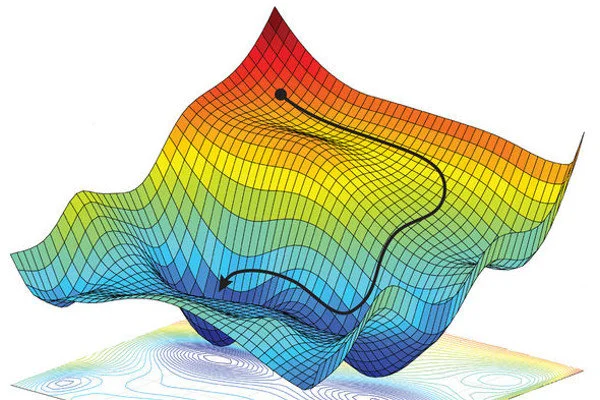
\includegraphics[width=\textwidth]{figures/gradient_descent}
    \end{columns}
\end{frame}

\begin{frame}
    \frametitle{Optimisation: Bayesian optimisation (for expensive functions)}
    \begin{columns}
        \column{0.5\textwidth}
        \begin{itemize}
            \item Best approach for punitively expensive functions
            \item Uses a Gaussian process to model the function, and propose the optimal new point which achieves an objective (e.g. maximisation), taking into account all uncertanties
            \item These are used to e.g. optimise hyperparameters in machine learning/N body simulations
        \end{itemize}
        
        \column{0.5\textwidth}
        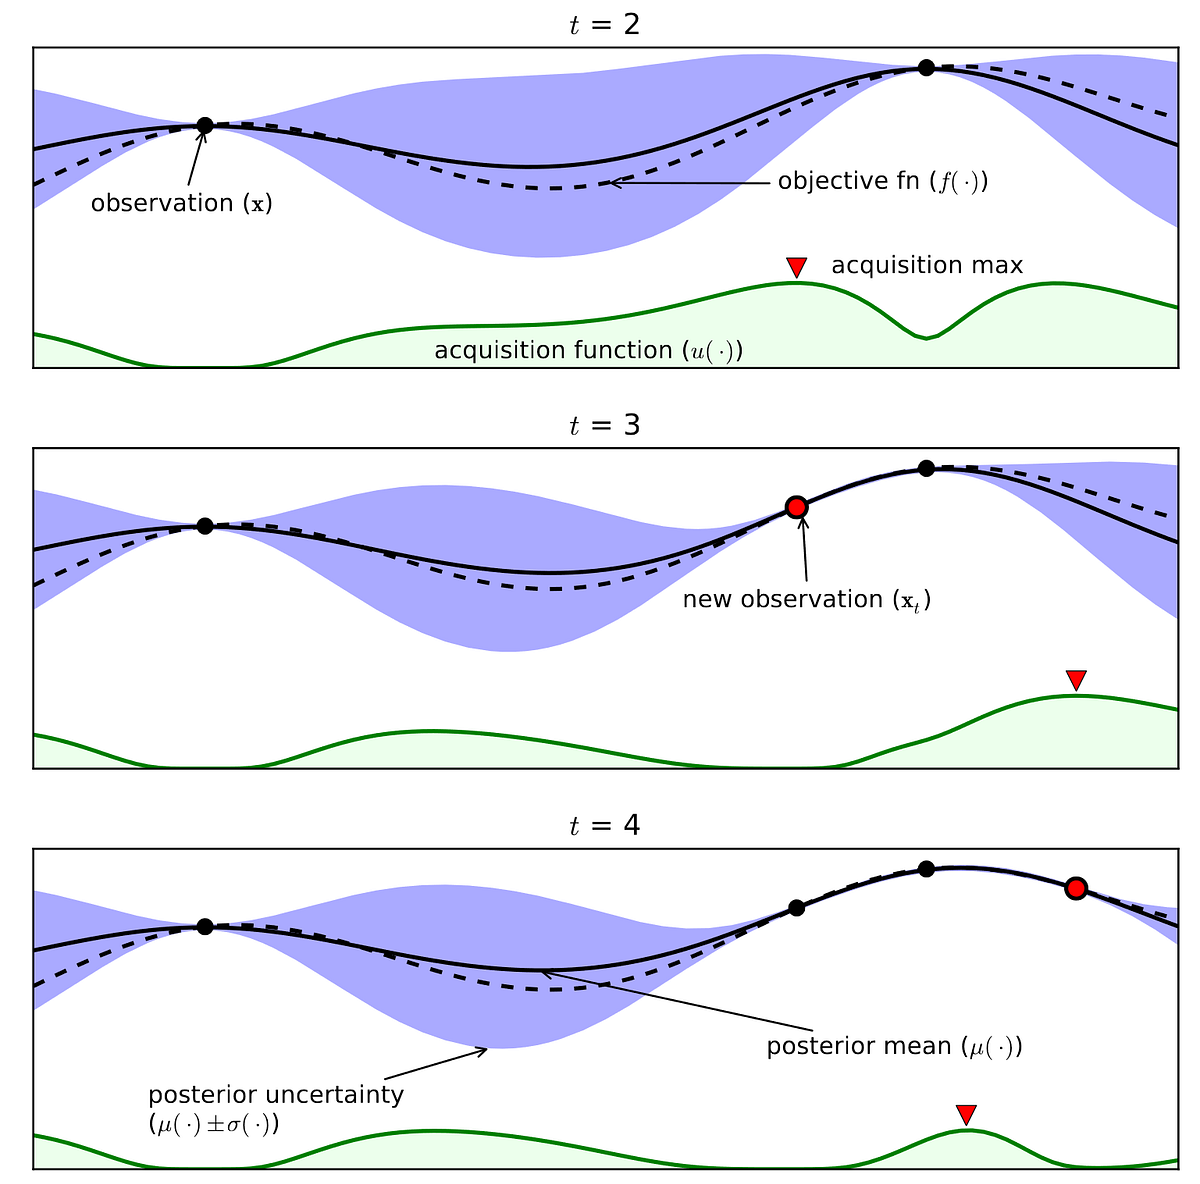
\includegraphics[width=\textwidth]{figures/bayesian_optimisation}
    \end{columns}
\end{frame}

\begin{frame}
    \frametitle{Optimisation: Genetic Algorithms (for profiling)}
    \begin{columns}
        \column{0.5\textwidth}
        \begin{itemize}
            \item Algorithms use an evolutionary process:
                \begin{itemize}
                    \item Generate a population of points
                    \item Reproduce: Recombine, mutate
                    \item Kill off low ranking points
                \end{itemize}
            \item \texttt{diver} is the genetic algorithm for differential evolution preferred by GAMBIT
            \item Generally accepted as being good for solving multimodal functions
            \item Not statistically principled or interpretable if it goes wrong
            \item These in practice are good for profiling in medium dimensions, since the evolutionary process generates many good candidate points -- but technically a global optimiser!
        \end{itemize}
        \column{0.5\textwidth}
        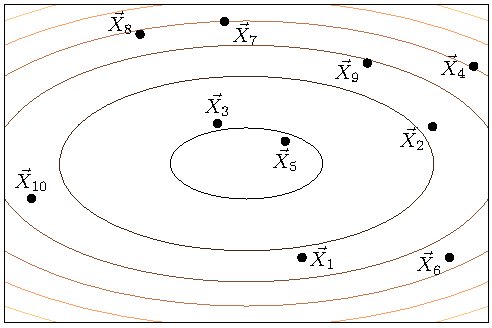
\includegraphics[width=0.5\textwidth]{figures/diver_1}%
        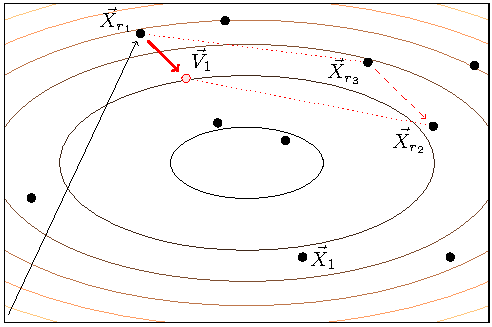
\includegraphics[width=0.5\textwidth]{figures/diver_2}
        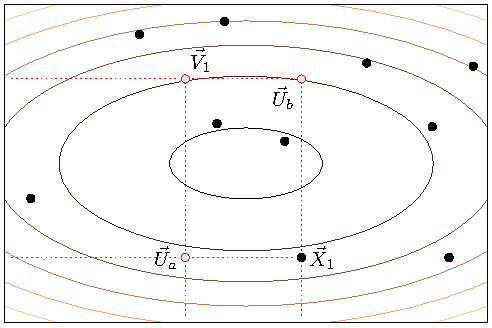
\includegraphics[width=0.5\textwidth]{figures/diver_3}%
        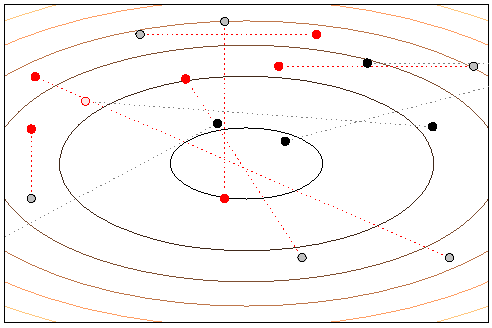
\includegraphics[width=0.5\textwidth]{figures/diver_4}
    \end{columns}
\end{frame}

%\begin{frame}
%    \frametitle{GAMBIT}
%    \begin{columns}
%        \column{0.4\textwidth}
%        \column{0.6\textwidth}
%        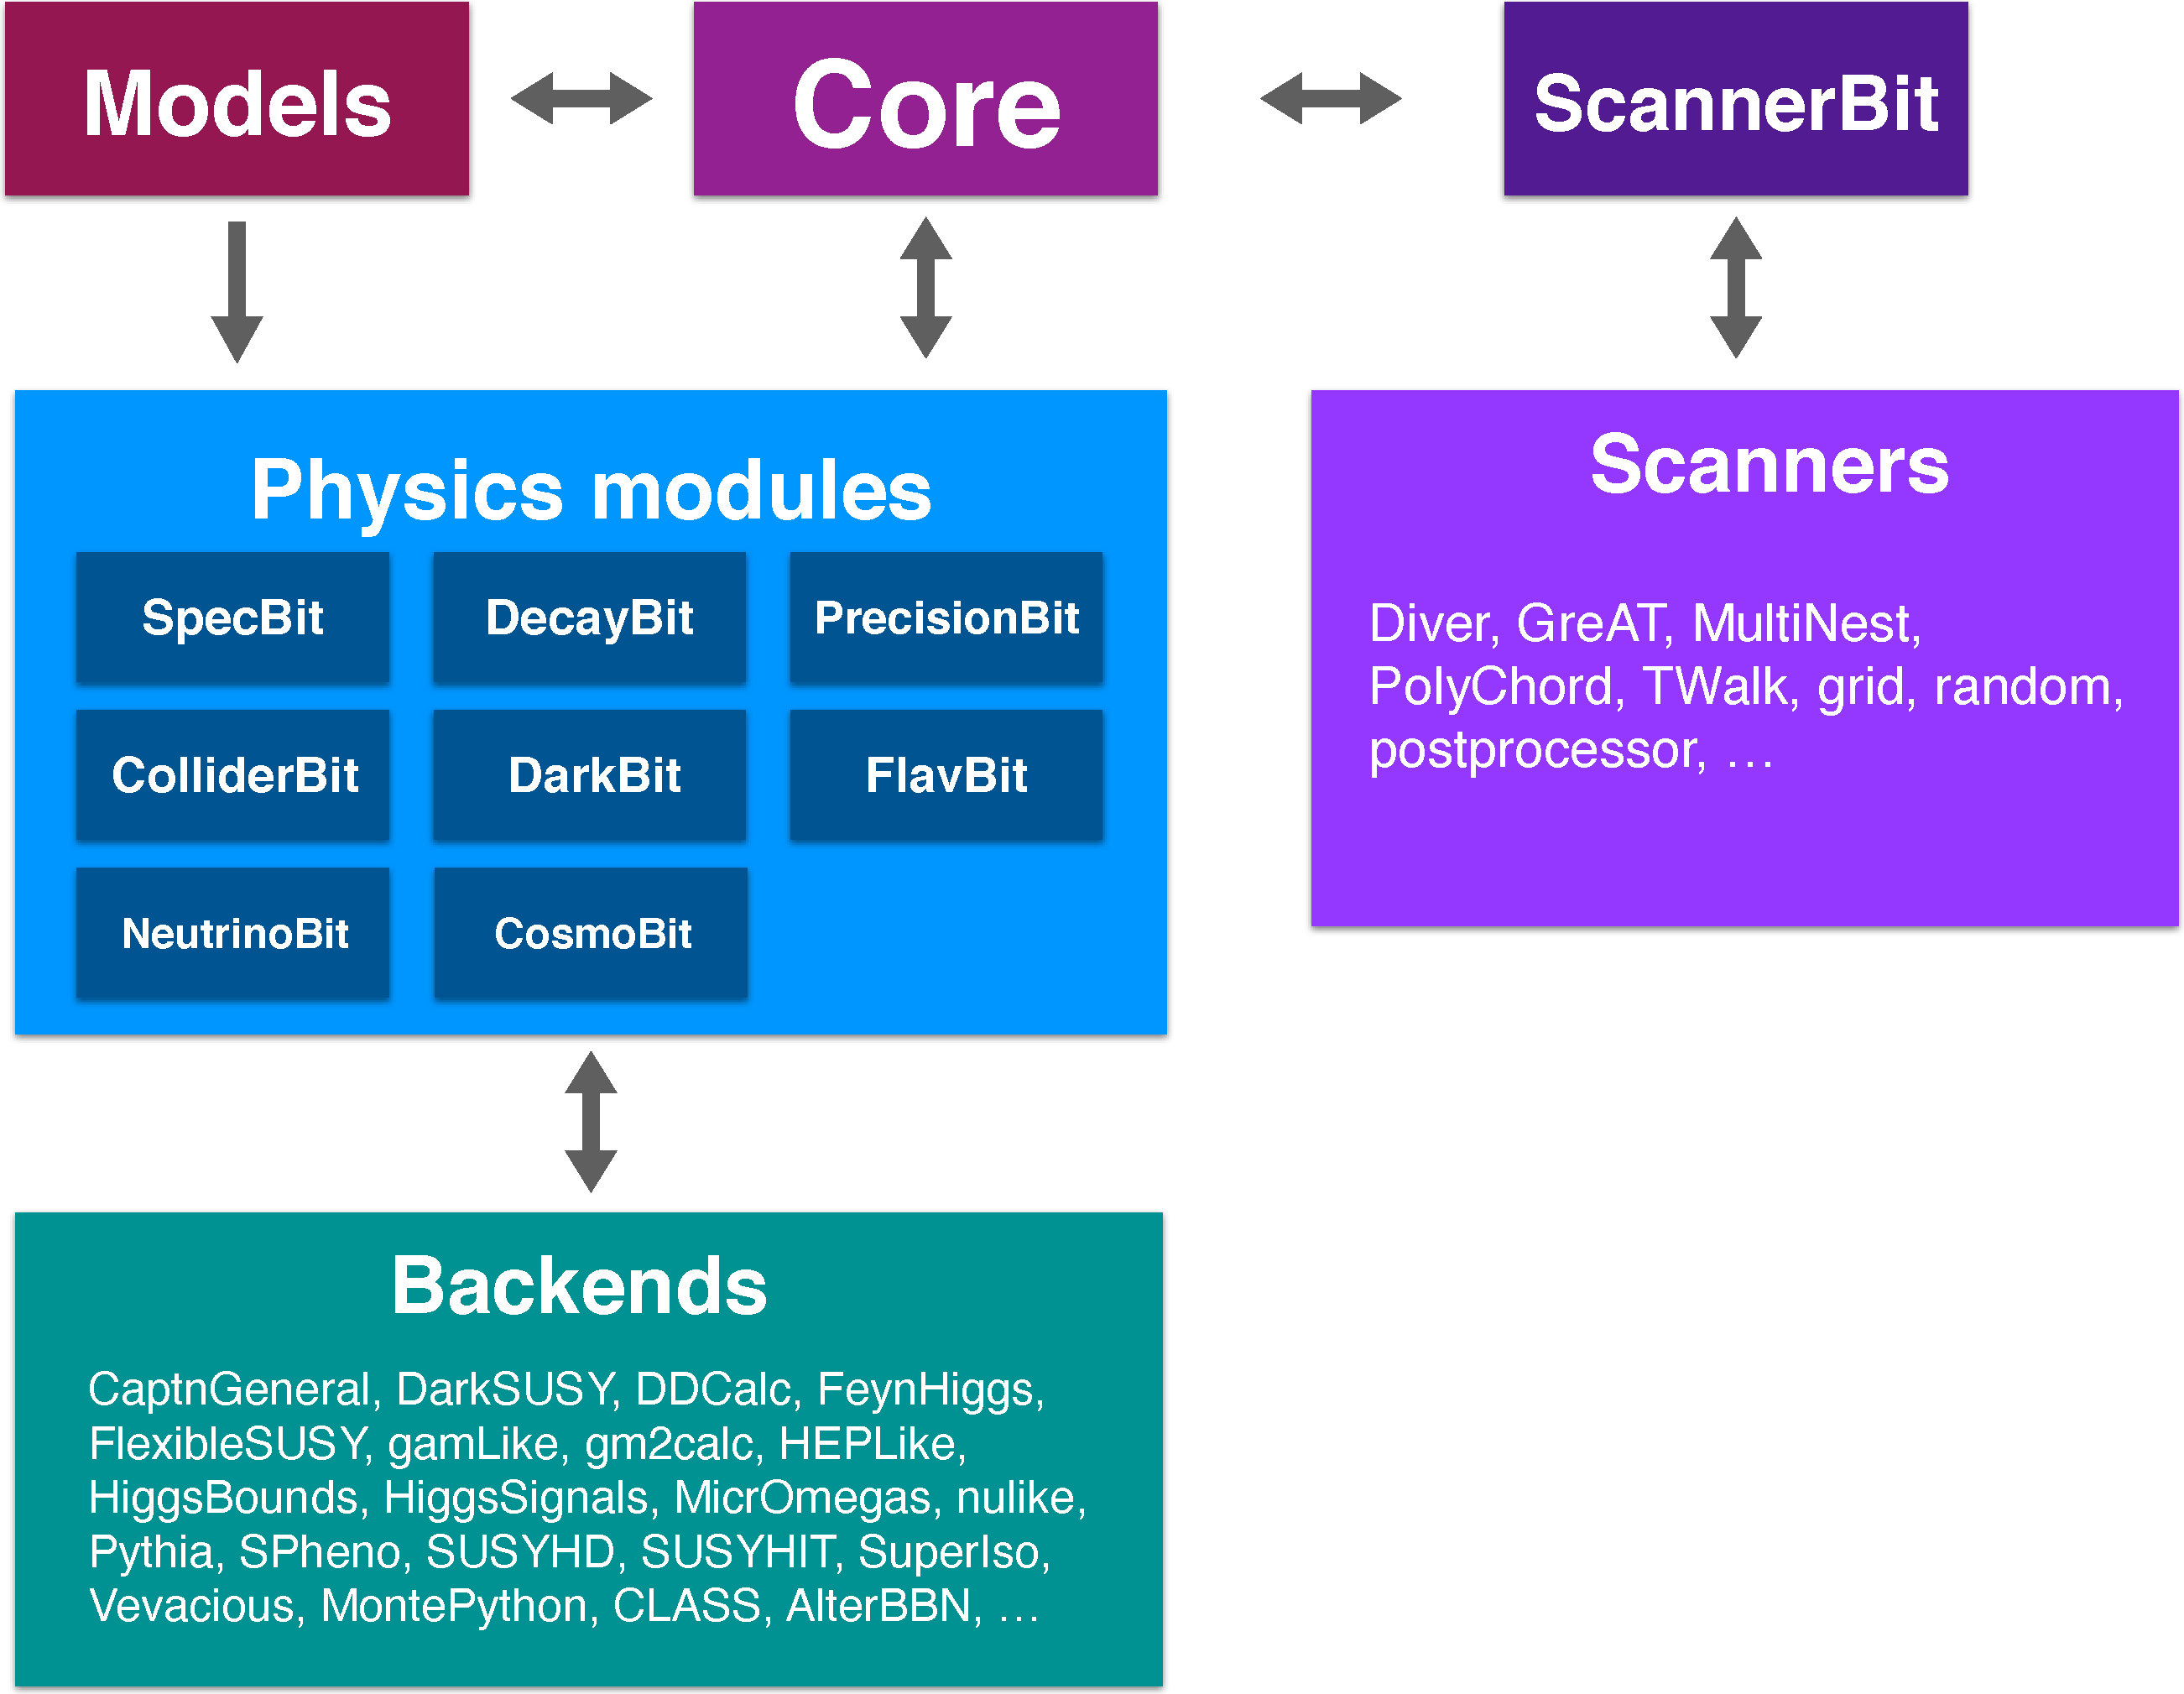
\includegraphics[width=\textwidth]{figures/gambit_layout}
%    \end{columns}
%\end{frame}



%\begin{frame}
%    \frametitle{Notation}
%    \begin{itemize}
%        \item Space of parameters $\theta$
%        \item Probability distribution/function $\mathcal{P}(\theta)$
%        \item Region of valid parameters/support of function/prior/measure $\pi(\theta)$
%            \begin{itemize}
%                \item Note that for any numerical method even if not specified there is an implicit measure imposed by floating point arithmetic
%            \end{itemize}
%    \end{itemize}
%\end{frame}




\begin{frame}
    \frametitle{Metropolis Hastings (baseline sampling algorithm)} 
    \begin{itemize}
        \item Turn the $N$-dimensional problem into a one-dimensional one.
        \item Pick start point $\theta_0$.
        \item At step $i$:
            \begin{enumerate}
                \item Propose a new point $\theta_{i+1}$ a small step away from $\theta_{i}$
                \item If uphill $\mathcal{P}(\theta_{i+1}) > \mathcal{P}(\theta_i)$, make step\ldots
                \item \ldots otherwise make step with probability $\alpha = \mathcal{P}(\theta_{i+1}) / \mathcal{P}(\theta_i)$. 
            \end{enumerate}
        \item Requires a proposal distribution $\mathcal{Q}(\theta_{i+1}|\theta_i)$
        \item In general case where $\mathcal{Q}$ is not symmetric, need acceptance ratio:
            \begin{equation*}
                \alpha = \frac{\mathcal{P}(\theta_{i+1})\mathcal{Q}(\theta_{i}|\theta_{i+1})}{\mathcal{P}(\theta_{i})\mathcal{Q}(\theta_{i+1}|\theta_{i})}
            \end{equation*}
    \end{itemize}
    \begin{block}{TOOLS}
        Whilst many exist: $\texttt{PyMC3}$, $\texttt{cobaya}$, $\texttt{MontePython}$,\ldots, in practice the algo is so simple, and the proposal distribution so problem-specific, it's usually relatively efficient to write your own.
    \end{block}
\end{frame}

\begin{frame}
    \frametitle{Metropolis Hastings } 
    \framesubtitle{Where can this go wrong?}
    \begin{itemize}
        \item Burn in
            \begin{itemize}
                \item It can take a while for the chain to equilibriate to the typical set
                \item It is hard to diagnose burn in, particularly in high dimensions
            \end{itemize}
        \item Multimodality
            \begin{itemize}
                \item If the function has multiple separated peaks, despite mathematical guarantees of convergence it will take a Hubble time to move between modes.
            \end{itemize}
        \item Correlated distributions
            \begin{itemize}
                \item In practice the peak(s) of the distribution have nontrivial structure (e.g. narrow ridges)
                \item Very hard to create a flexible enough proposal to accomodate all, and not strictly Markovian
            \end{itemize}
        \item Phase transitions
            \begin{itemize}
                \item A different kind of multi-modality, which can occur if the function is a ``slab and spike''
                \item Two regions -- one high-volume $V$ lower $\mathcal{P}$, the other low $V$ high $\mathcal{P}$. Difficult to transition
            \end{itemize}
        \item Poor parallelisation
            \begin{itemize}
                \item In practice it is not well parallelised, since majority of time is spent in burn-in
            \end{itemize}
    \end{itemize}
\end{frame}



\begin{frame}
    \frametitle{Hamiltonian Monte-Carlo (ultra high dimensional sampling)} 
    \begin{itemize}
        \item Key idea: Treat $\log L(\Theta)$ as a potential energy
        \item Guide walker under ``force'': \[F(\Theta) =-\nabla \log L(\Theta)\]
        \item Walker is naturally ``guided'' uphill
        \item Conserved quantities mean efficient acceptance ratios.
        \item Whilst the recieved wisdom is that this is ``tuning parameter free'', in practice the mass matrix has similar degrees of tuning unless the problem is already normalised (physicists naturally do this, which explains why it works so well out of the box).
            \begin{block}{TOOLS}
                \item \texttt{stan} is a fully fledged, mature programming language with HMC as a default sampler.
                \item \texttt{TensorFlow}, \texttt{PyTorch} \& \texttt{JAX} all have HMC implementations.
            \end{block}
    \end{itemize}
\end{frame}

\begin{frame}
    \frametitle{Ensemble sampling (robust alternative to MH)} 
    \begin{itemize}
        \item Instead of one walker, evolve a set of $n$ walkers.
        \item Can use information present in ensemble to guide proposals.
        \item Generally tuning parameter free
        \item Struggles with multimodal distributions
        \item Strive to be affine invariant
    \begin{block}{TOOLS}
        \begin{itemize}
            \item \texttt{emcee}: The MCMC Hammer~\arxiv{1202.3665}
            \item \texttt{zeus}: Ensemble slice sampling~\arxiv{2002.06212}
        \end{itemize}
    \end{block}
    \end{itemize}
\end{frame}

%\begin{frame}
%    \frametitle{The fundamental issue with all of the above} 
%
%    \begin{itemize}
%        \item They can't integrate functions over the space
%            \begin{align}
%                Z
%                &= P(D|M) 
%                \nonumber\\
%                &= \int P(D|\Theta,M)P(\Theta|M) d\Theta 
%                \nonumber\\
%                &= \left\langle L \right\rangle_\pi
%                \nonumber
%            \end{align}
%        \item MCMC fundamentally explores the posterior, and cannot average over the prior.
%        \item Simulated annealing gives one possibility for ``tricking'' MCMC into computing evidences.
%            \begin{itemize}
%                \item Inspired by thermodynamics.
%                \item Suffers from similar issues to MCMC.
%                \item Unclear how to choose correct annealing schedule
%            \end{itemize}
%    \end{itemize}
%
%\end{frame}


\begin{frame}
    \frametitle{Nested sampling (high dimensional integration)}
    \begin{columns}
        \column{0.5\textwidth}
        \begin{itemize}
            \item Start with $n$ random samples over the space.
            \item Delete outermost sample, and replace with a new random one at higher integrand value.
            \item The ``live points'' steadily contract around the peak(s) of the function.
            \item We can use this evolution to estimate volume \emph{probabilistically}.
            \item At each iteration, the contours contract by $\sim\frac{1}{n}\only<9->{\pm \frac{1}{n}}$ of their volume.
            \item This is an exponential contraction, so
                \[  \int f(x) dV \approx \sum_i f(x_i) \Delta V_i, \quad V_i = V_0 e^{-\only<9->{(}i\only<9->{\pm\sqrt{i})}/n} \]
%            \item Nested sampling: completely different way to scan.
%            \item Ensemble sampling compresses entire space$\to$peak(s).
%            \item Sequentially update a set $S$ of $n$ samples:
%                \begin{itemize}
%                    \item[$S_0$:]  Generate $n$ samples uniformly over the space (from a measure $\pi$). 
%
%                    \item[$S_{i+1}$:] Delete the lowest likelihood sample in $S_{i}$, and replace it with a new uniform sample with higher likelihood.
%                \end{itemize}
%            \item Requires one to be able to sample uniformly within a region, subject to a {\em hard constraint}:
%                \[\{\theta\sim \pi : \mathcal{L}(\theta)>\mathcal{L}_*. \}\]
%            \item This procedure optimises (multimodally), and can calculate the \C[3]{evidence}/integral of function \& \C[0]{posterior}/sample weights.
        \end{itemize}
        \column{0.5\textwidth}
        \includegraphics<1|handout:0>[width=\textwidth,page=1]{figures/himmelblau}%
        \includegraphics<2|handout:0>[width=\textwidth,page=2]{figures/himmelblau}%
        \includegraphics<3|handout:0>[width=\textwidth,page=3]{figures/himmelblau}%
        \includegraphics<4|handout:0>[width=\textwidth,page=4]{figures/himmelblau}%
        \includegraphics<5|handout:0>[width=\textwidth,page=5]{figures/himmelblau}%
        \includegraphics<6|handout:0>[width=\textwidth,page=6]{figures/himmelblau}%
        \includegraphics<7|handout:0>[width=\textwidth,page=7]{figures/himmelblau}%
        \includegraphics<8-         >[width=\textwidth,page=8]{figures/himmelblau}%
    \end{columns}
\end{frame}

%\begin{frame}
%    \frametitle{The nested sampling meta-algorithm: dead points}
%    \begin{columns}
%        \column{0.5\textwidth}
%        \begin{itemize}
%            \item At the end, one is left with a set of discarded ``dead'' points.
%            \item Can be weighted to form posterior samples, prior samples, or anything in between.
%            \item Nested sampling estimates the \textbf{density of states} and calculates partition functions
%                \[Z(\beta) = \sum_i f(x_i)^\beta \Delta V_i.\]
%            \item The evolving ensemble of live points allows:
%                \begin{itemize}
%                    \item implementations to self-tune
%                    \item exploration of multimodal functions
%                    \item global and local optimisation
%                \end{itemize}
%            %\item Interpreted as a Bayesian algorithm, it
%            %    \begin{itemize}
%            %        \item Computes the Bayesian evidence (model comparison)
%            %        \item Produces (weighted) posterior samples (parameter estimation)
%            %    \end{itemize}
%        \end{itemize}
%        \column{0.5\textwidth}
%        \includegraphics[width=\textwidth,page=14]{figures/himmelblau}%
%        %\includegraphics<1|handout:0>[width=\textwidth,page=14]{figures/himmelblau}%
%        %\includegraphics<2          >[width=\textwidth,page=15]{figures/himmelblau}%
%    \end{columns}
%\end{frame}

\begin{frame}
    \frametitle{The dead measure~\arxiv{2312.00294}}
    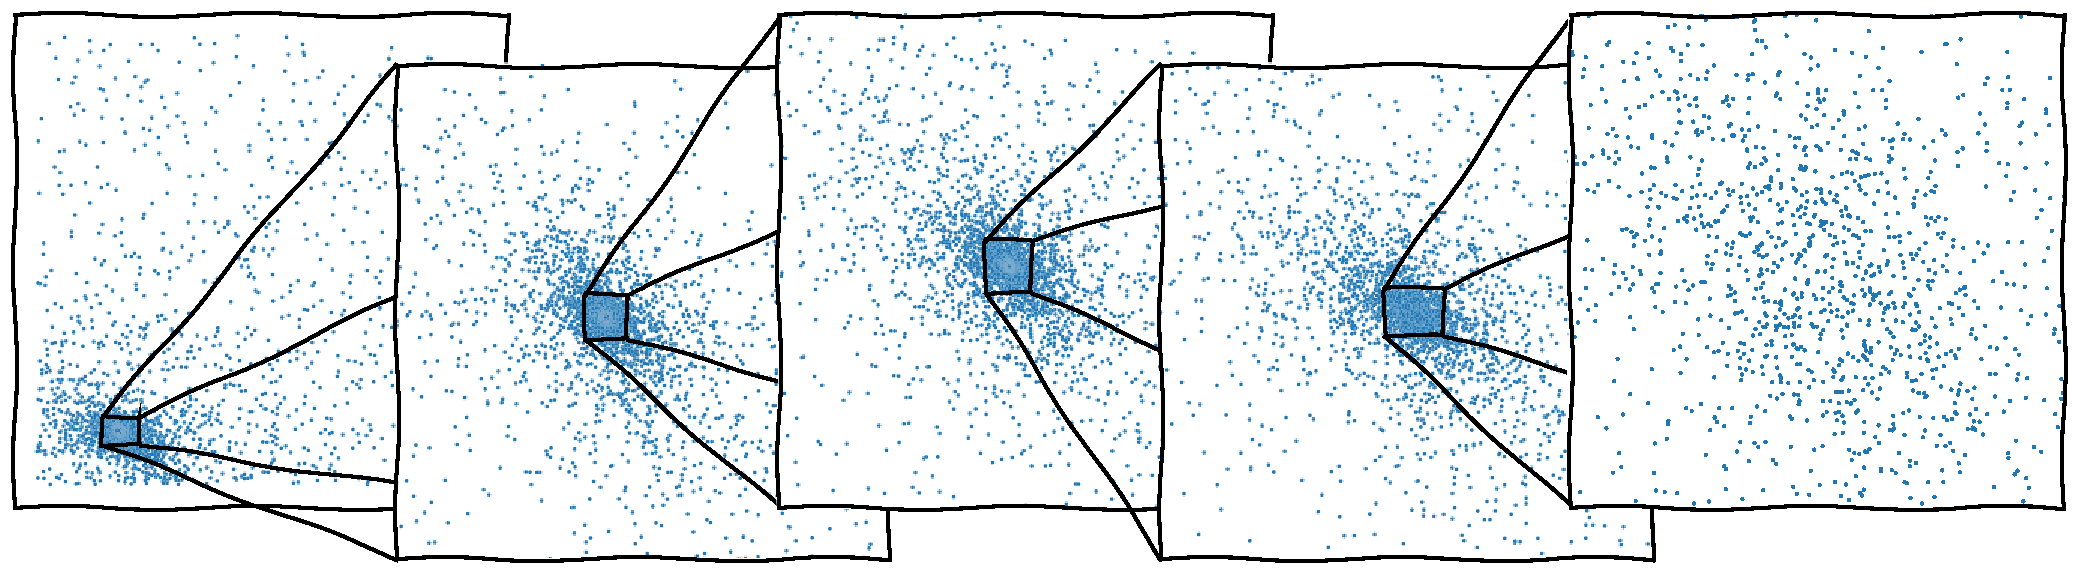
\includegraphics[width=\textwidth]{figures/dead_measure}
    \begin{columns}
        \column{0.69\textwidth}
        \begin{itemize}
            \item Dead points have a unique scale-invariant distribution $\propto\: \tfrac{dV}{V}$.
            \item Uniform over original region, exponentially concentrating on region of interest (until termination volume).
            \item Full coverage of tails enables integration.
            \item Good for training emulators (HERA~\arxiv{2108.07282}).
        \end{itemize}
        \column{0.3\textwidth}
        \begin{block}{Applications}
        \begin{itemize}
            \item training emulators.
            \item gridding simulations
            \item beta flows\ldots
            \item good name for a band
        \end{itemize}
        \end{block}
    \end{columns}
\end{frame}

\begin{frame}
    \frametitle{Implementations of Nested Sampling \arxiv{2205.15570}(NatReview)}
    %\begin{columns}
    %    \begin{column}{0.33}
    %        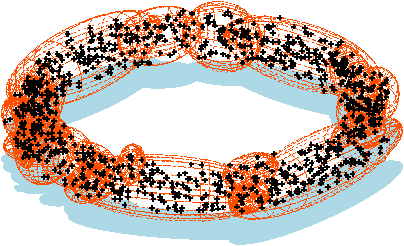
\includegraphics[width=\textwidth]{figures/multinest}
    %    \end{column} 
    %\end{columns}
    \begin{columns}[t]
        \column{0.3\textwidth}
        \texttt{MultiNest}~\arxiv{0809.3437}
        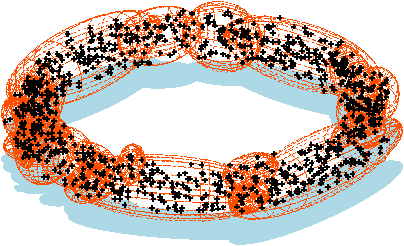
\includegraphics[width=\textwidth]{figures/multinest}
        \texttt{UltraNest}~\arxiv{2101.09604}
        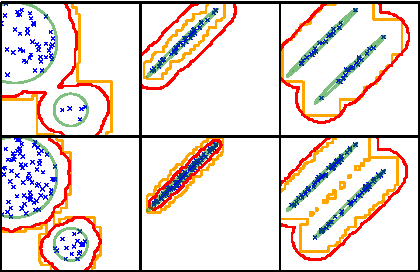
\includegraphics[width=\textwidth]{figures/radfriends}
        \column{0.4\textwidth}
        \texttt{PolyChord}~\arxiv{1506.00171}
        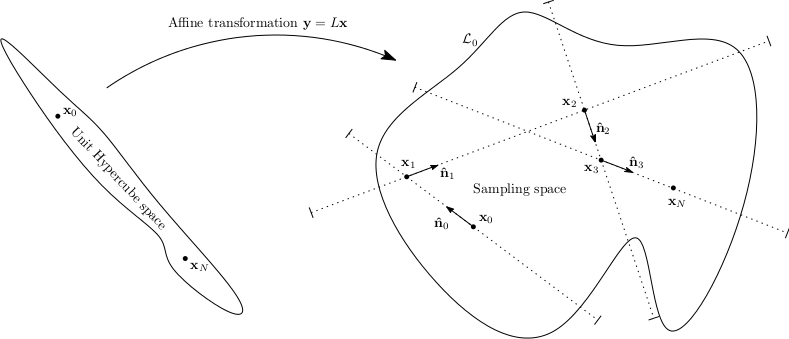
\includegraphics[width=\textwidth]{figures/polychord}
        \vfill
        \texttt{NeuralNest}~\arxiv{1903.10860}
        \begin{columns}
            \column{0.5\textwidth}
            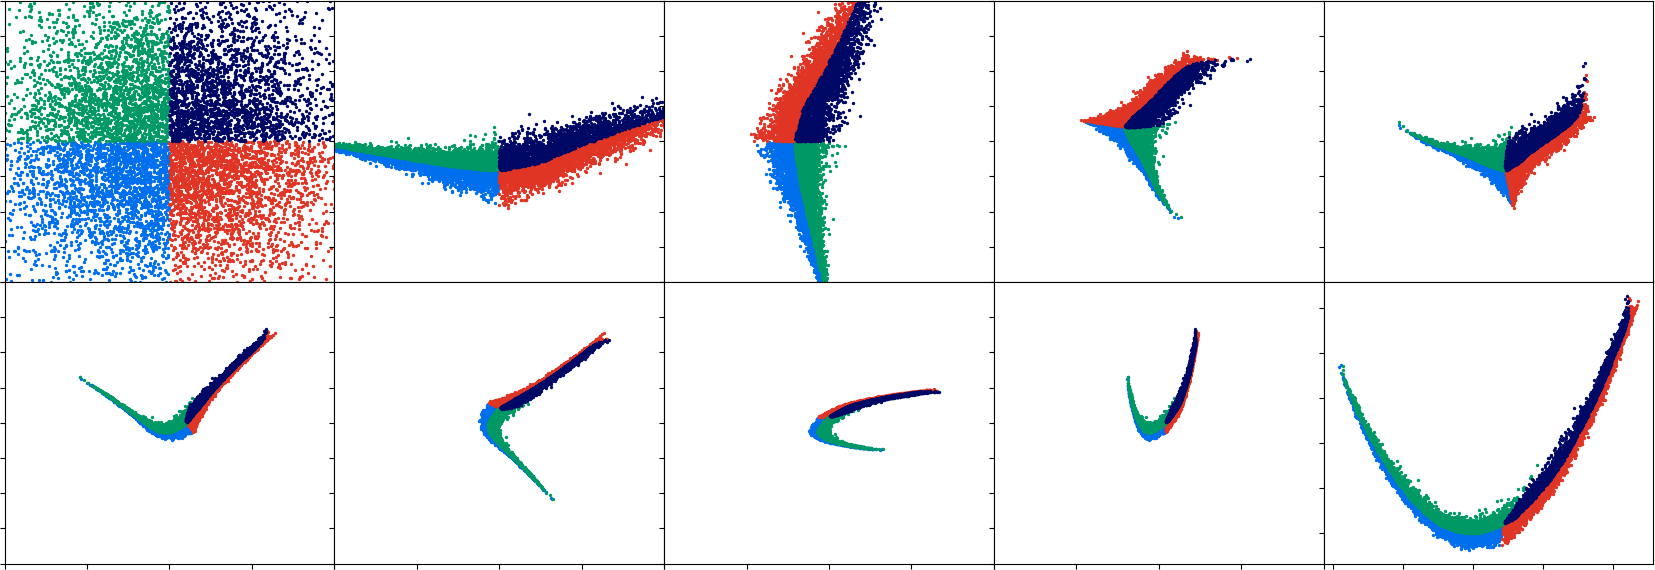
\includegraphics[width=\textwidth]{figures/rosenbrock_flow.png}
            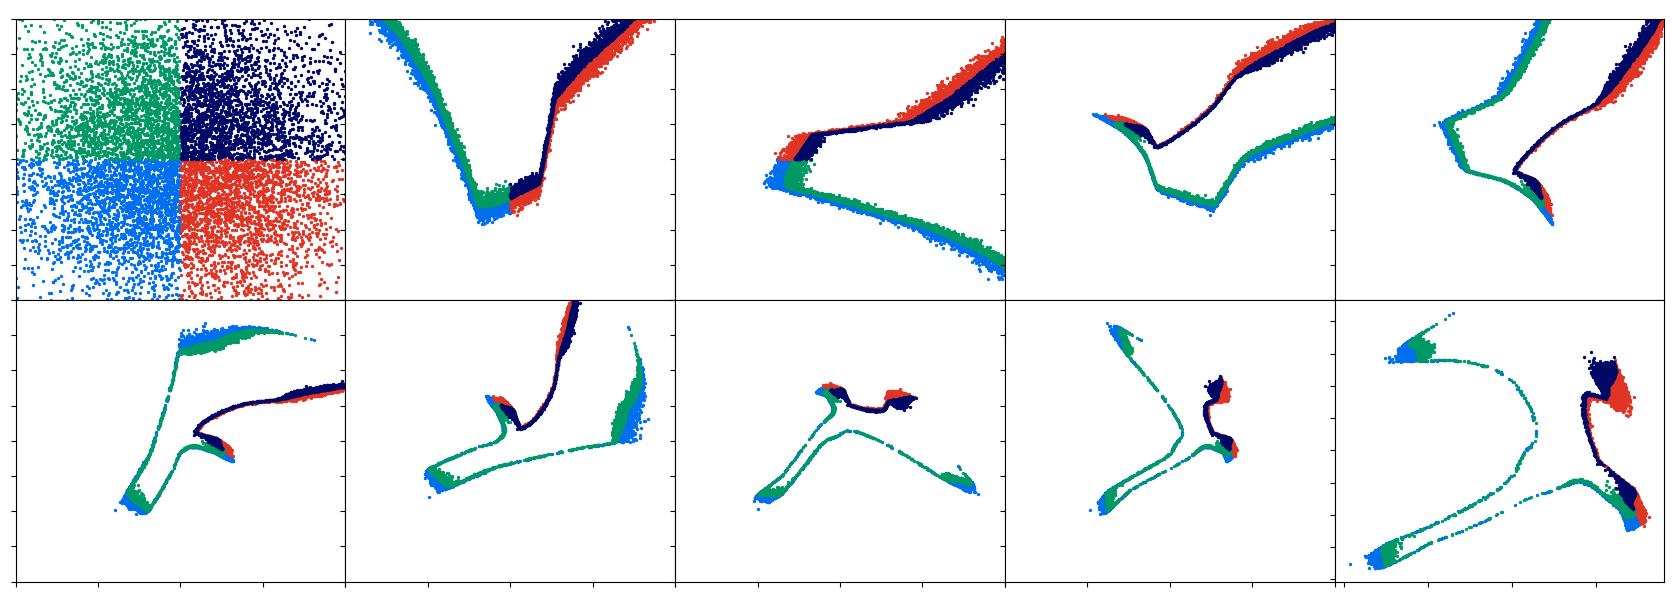
\includegraphics[width=\textwidth]{figures/himmelblau_flow.png}
            \column{0.5\textwidth}
            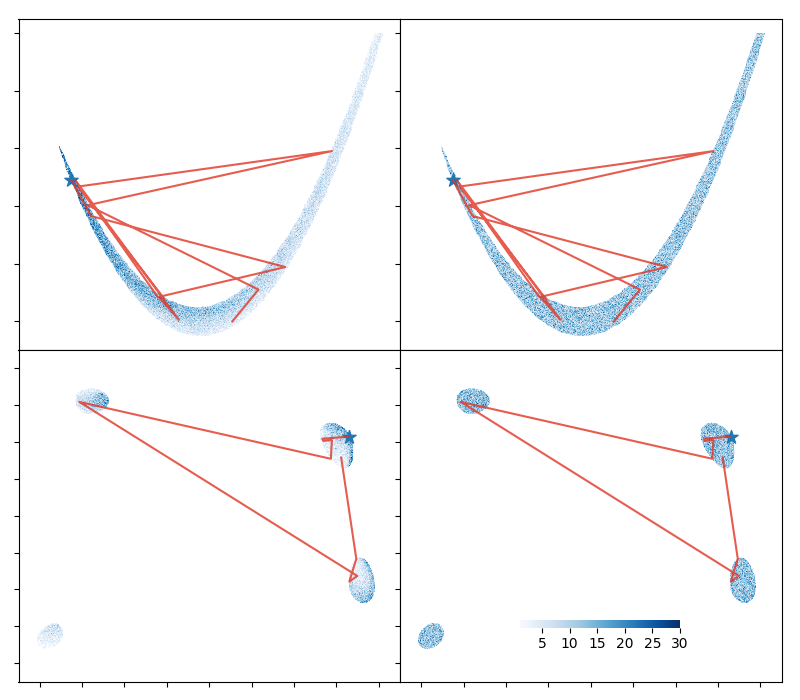
\includegraphics[width=\textwidth]{figures/chains.png}
        \end{columns}
        \texttt{nessai}~\arxiv{2102.11056} \texttt{nora}~\arxiv{2305.19267}
        \vfill
        \column{0.3\textwidth}
        \texttt{DNest}~\arxiv{1606.03757}
        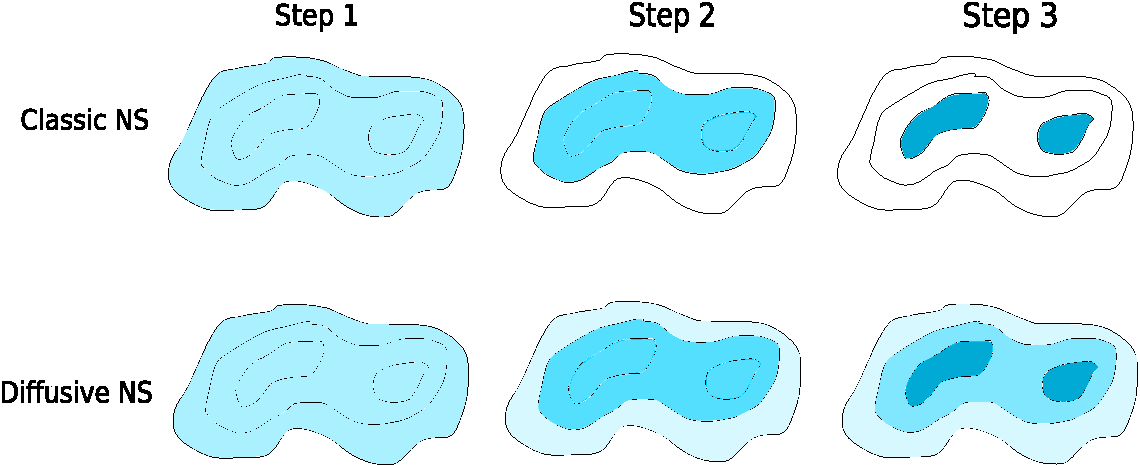
\includegraphics[width=\textwidth]{figures/dnest}
        \texttt{ProxNest}~\arxiv{2106.03646}
        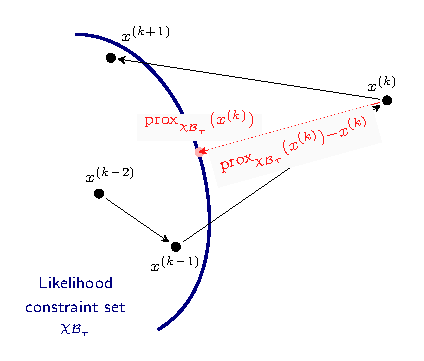
\includegraphics[width=\textwidth]{figures/proxnest_diagram}
        \texttt{dynesty}~\arxiv{1904.02180} 
        \vfill
    \end{columns}
\end{frame}


%\begin{frame}
%    \frametitle{Likelihood free inference}
%    <+Content+>
%\end{frame}






\begin{frame}
    \frametitle{Software frameworks}
    \begin{columns}
        \column{0.5\textwidth}
        \begin{itemize}
            \item Principled scientific data analysis requires a lot of different components:
                \begin{itemize}
                    \item Data
                    \item Theory
                    \item Statistics
                    \item Likelihoods
                    \item Samplers/scanners
                    \item Post-processing
                \end{itemize}
            \item Mature communities develop frameworks to do all of the above in one go:
                \begin{itemize}
                    \item Cosmology: \texttt{CosmoMC}, \texttt{MontePython}, \texttt{Cobaya}, \texttt{CosmoSIS}, \texttt{CosmoLike}
                    \item Gravitational Waves : \texttt{LAL}, \texttt{Bilby}, \texttt{PyCBC}
                    \item Particle physics: \texttt{GAMBIT}, \texttt{MasterCode}
                \end{itemize}
            \item Much harder if you want to combine data from multiple communities
        \end{itemize}
        \column{0.5\textwidth}
        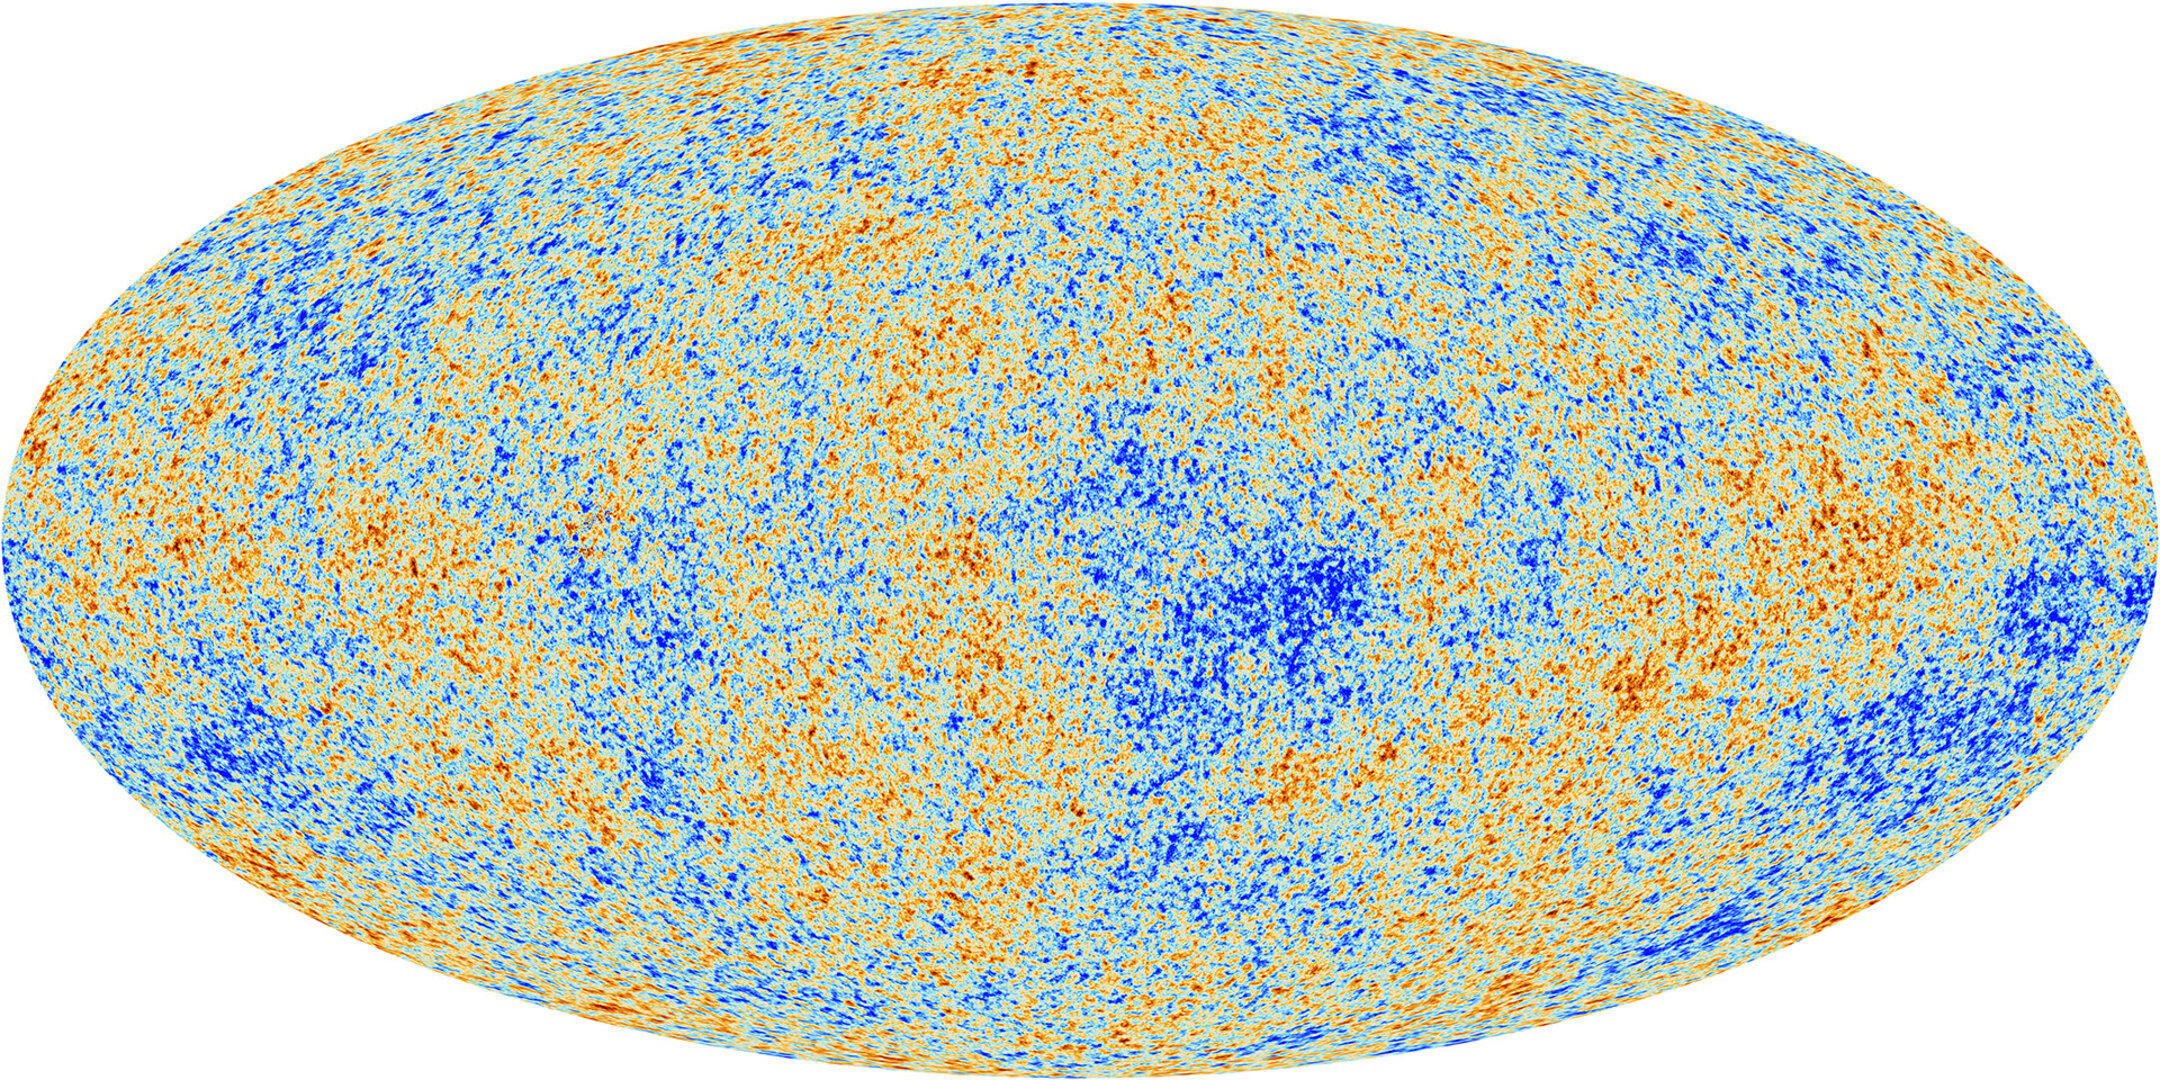
\includegraphics[width=0.5\textwidth]{figures/cmb}%
        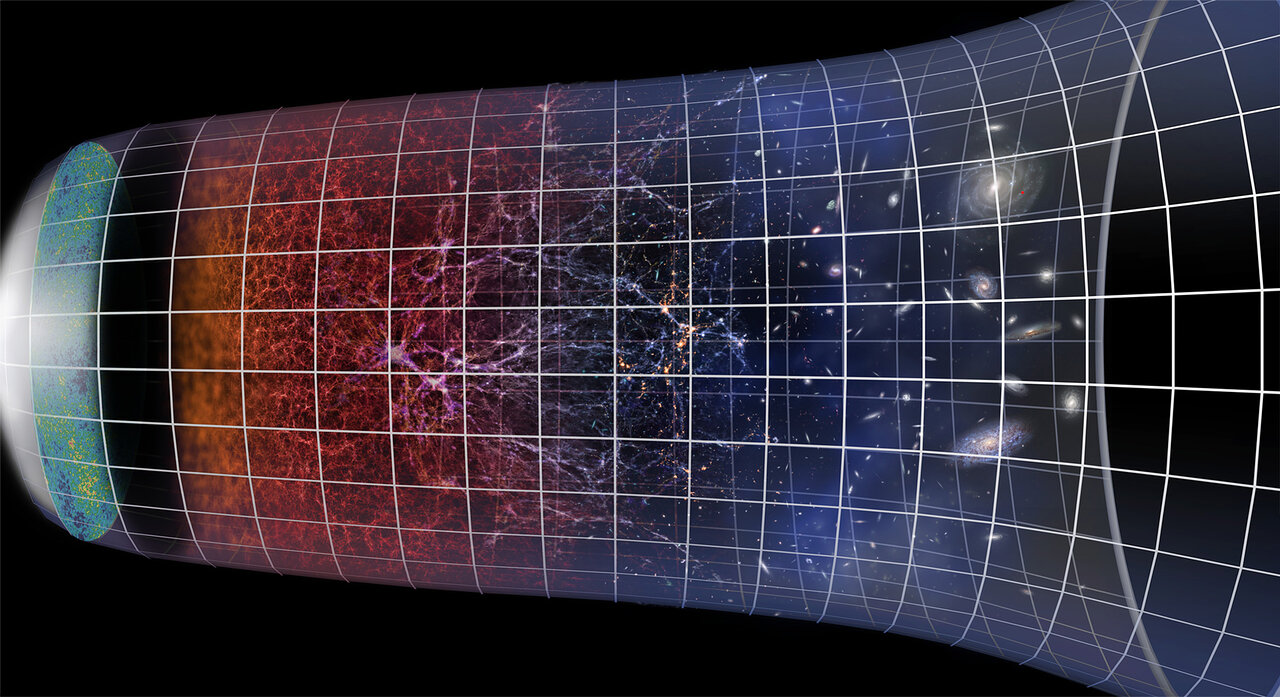
\includegraphics[width=0.5\textwidth]{figures/theory}
        \begin{columns}
            \column{0.55\textwidth}
        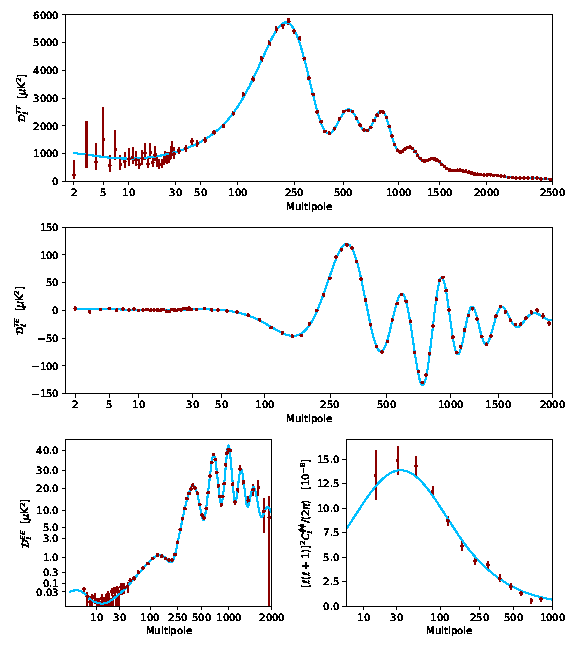
\includegraphics[width=\textwidth]{figures/coadded}%
            \column{0.45\textwidth}
        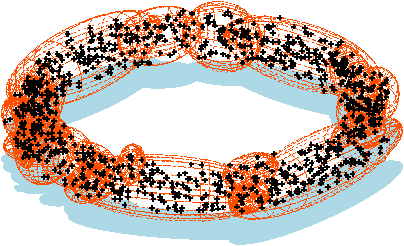
\includegraphics[width=\textwidth]{figures/multinest}%

        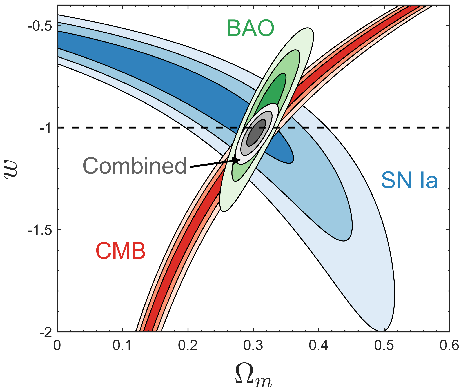
\includegraphics[width=\textwidth]{figures/parameters}
            
        \end{columns}
    \end{columns}
\end{frame}

{
    \usebackgroundtemplate{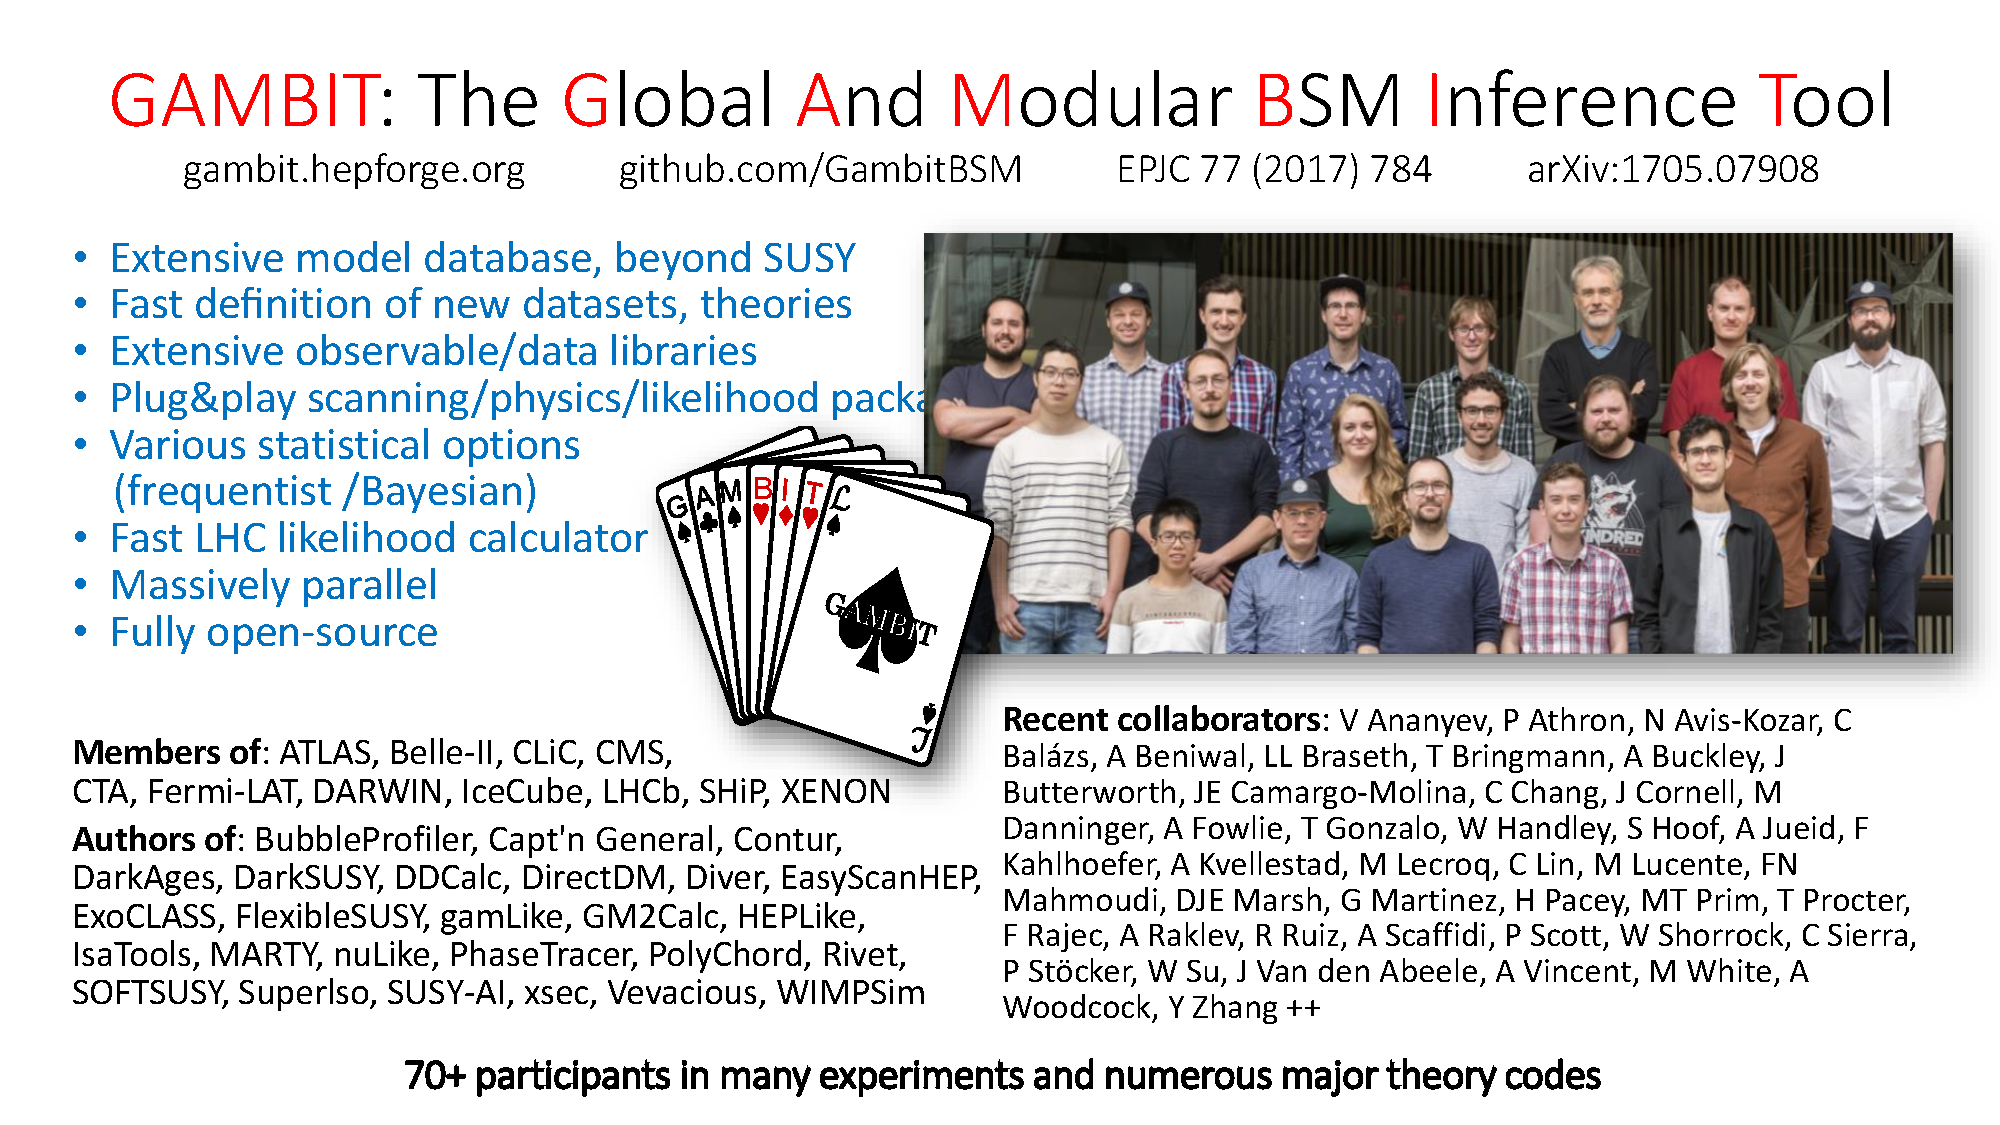
\includegraphics[width=\paperwidth]{gambit_ad_slide}}
    \begin{frame}[plain]
    \end{frame}
}

\begin{frame}
    \frametitle{What is GAMBIT?}
    \vspace{-10pt}
    \begin{columns}[t]
        \column{0.48\textwidth}
        \begin{block}{GAMBIT as a software framework}
            \begin{itemize}
                \item Combines collider, direct detection, neutrino \& telescope data.
                \item Allows joint analysis of dark matter, neutrinos \& BSM physics
                \item MPI + OpenMP parallelisation \\(record of 115,000 CPUs)
                \item Combines libraries \& codes written in:\\
                    \texttt{C++}, \texttt{Fortran}, \texttt{Python}, \texttt{Mathematica}\ldots
                \item Highly modular ``Bits''
                \item Often with several alternatives
            \end{itemize}
        \end{block}
        \column{0.48\textwidth}
        \begin{block}{GAMBIT as a community}
            \begin{itemize}
                \item Particle physicists, cosmologists \& statisticians ($>$80 members)
                \item Generates interdisciplinary expertise \& inspires new techniques
                \item Open source software
                \item Access to large community computing resources (40MCPUh/y)
                \item Modularity allows parallel teams
                \item Short-author papers by default
                \item in-person meetings every 9 months
            \end{itemize}
        \end{block}
    \end{columns}


%Greg

% More slides
% https://www.dropbox.com/s/2c7c475t6traj42/Data_at_UiO_2022_Kvellestad.pdf?dl=0

%Anders:
    % talk to atlas susy group
    % trivial point which landed well: if we're going to use a smart sampling algorithm, then parallelisation will be non-trivial
    % atlas recently released pmssm, completely random sampling, so they can do sampling, and then parallelised physics computations in increasing levels of complexity offline after the sampling
    % adaptive sampling algorithms _require_ all likelihood computations on the fly.
    % at the end of the day they just classify points as excluded or not
    % https://ui.adsabs.harvard.edu/abs/2022AAS...24030220M/abstract
    % https://www.overleaf.com/9325782714mghdvzmzxtpt#ba83d1
    
\end{frame}

\begin{frame}
    \frametitle{What is GAMBIT not?}
    \begin{columns}
        \column{0.65\textwidth}
        \begin{itemize}
            \item GAMBIT is not pip-installable
            \item It should be viewed as a ``power tool'' for heavy tasks
            \item Designed with HPC in mind 
                \begin{itemize}
                    \item expectation that forward modelling for frontier science takes seconds to hours
                \end{itemize}
            \item Combining data, theory \& code across multiple communities is non trivial
            \item Installing on a new system takes patience
                \begin{itemize}
                    \item Stickers for newcomers!
                \end{itemize}
        \end{itemize}
        \column{0.35\textwidth}
        
\includegraphics[width=\textwidth]{figures/gambit_sticker}
    \end{columns}

\end{frame}

\begin{frame}[fragile]
    \frametitle{ScannerBit~\arxiv{1705.07959}}
    \begin{columns}
        \column{0.5\textwidth}
        Original paper:
        \begin{itemize}
            \item describes code design \& structure
            \item compares performance of the main two scanning algorithms: \texttt{diver} \& \texttt{MultiNest}
                \begin{itemize}
                    \item also compared \texttt{Great}(MH) and \texttt{Twalk}(affine~invariant) 
                \end{itemize}
            \item Discusses Frequentist \& Bayesian analyses
            \item 15D MSSM scalar singlet (2+13 parameters)
            \item Modular \& flexible plugins homogenise scanning algorithms (agnostic of model/prior)
        \end{itemize}
        
        \column{0.5\textwidth}
        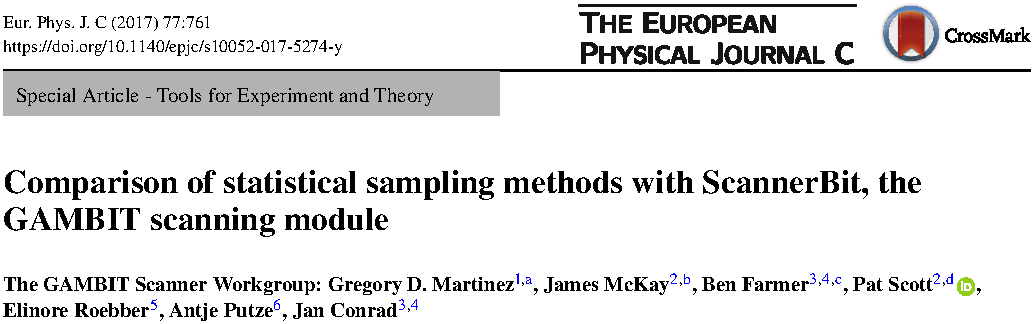
\includegraphics[width=\textwidth]{figures/scannerbit_header}
        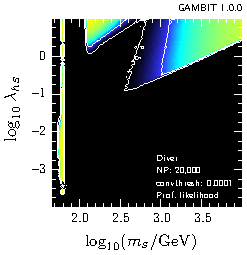
\includegraphics[width=0.5\textwidth]{figures/scannerbit_15d_diver_profile}%
        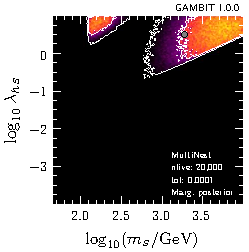
\includegraphics[width=0.5\textwidth]{figures/scannerbit_15d_mn_posterior}
    \end{columns}
\end{frame}

\begin{frame}[fragile]
    \frametitle{ScannerBit 2.0}
    \begin{columns}
        \column{0.5\textwidth}
        Developments since original ScannerBit paper:
        \begin{enumerate}
            \item New scanning algorithms
                \begin{itemize}
                    \item \texttt{MINUIT2}
                    \item \texttt{PolyChord}
                    \item particle swarm
                \end{itemize}
            \item \texttt{PyScannerBit}
                \begin{itemize}
                    \item Isolation of scanners from GAMBIT
                    \item documentation: \href{https://pyscannerbit.readthedocs.io}{pyscannerbit.readthedocs.io}
                \end{itemize}
            \item Python Scanners
                \begin{itemize}
                    \item Allows easy incorporation of new scanning algorithms into GAMBIT
                    \item Modern machine learning techniques
                    \item (embarassingly) easy to incorporate
                \end{itemize}
        \end{enumerate}
        \begin{itemize}
            \item Paper release later this year.
            \item Beta testers welcome! \tiny{\href{mailto:gambit-scan@projects.hepforge.org}{gambit-scan@projects.hepforge.org}}
        \end{itemize}
        \column{0.5\textwidth}
\begin{lstlisting}[language=Python]
"""scipy.optimize scanner."""
import scanner_plugin as splug
import scipy.optimize
import numpy as np


class Minimize(splug.scanner):
    __version__ = scipy_version

    def __init__(self, **kwargs):
        super().__init__(use_mpi=False,
                         use_resume=False)

    def run(self):
        start = np.random.rand(self.dim)
        bounds = [(0., 1.)] * self.dim

        def neg_loglike_hypercube(x):
            return -self.loglike_hypercube(x)

        res = scipy.optimize.minimize(
                  neg_loglike_hypercube,
                  start, bounds=bounds)

        return 0

__plugins__ = {"scipy_minimize": Minimize}
\end{lstlisting}
    \end{columns}
\end{frame}

\begin{frame}[fragile]
    \frametitle{ScannerBit 2.0}
    \begin{columns}
        \column{0.5\textwidth}
        Developments since original ScannerBit paper:
        \begin{enumerate}
            \item New scanning algorithms
                \begin{itemize}
                    \item \texttt{MINUIT2}
                    \item \texttt{PolyChord}
                    \item particle swarm
                \end{itemize}
            \item \texttt{PyScannerBit}
                \begin{itemize}
                    \item Isolation of scanners from GAMBIT
                    \item documentation: \href{https://pyscannerbit.readthedocs.io}{pyscannerbit.readthedocs.io}
                \end{itemize}
            \item Python Scanners
                \begin{itemize}
                    \item Allows easy incorporation of new scanning algorithms into GAMBIT
                    \item Modern machine learning techniques
                    \item (embarassingly) easy to incorporate
                \end{itemize}
        \end{enumerate}
        \begin{itemize}
            \item Paper release later this year.
            \item Beta testers welcome! \tiny{\href{mailto:gambit-scan@projects.hepforge.org}{gambit-scan@projects.hepforge.org}}
        \end{itemize}
        \column{0.5\textwidth}
\begin{lstlisting}[language=Python]
"""Grid scanner with MPI."""
import scanner_plugin as splug
from utils import MPI
import numpy as np

class Grid(splug.scanner):

    __version__="1.0.0"

    def __init__(self, grid_pts=10, parameters=[],
                 **kwargs):
        super().__init__(use_mpi=True, use_resume=False)
        # Set up grid
        for param in self.parameter_names:
            n = grid_pts[parameters.index(param)]
            self.vecs.append(np.linspace(0.0, 1.0, n))
    
    def run(self):
        # Loop over grid with MPI
        grid = np.meshgrid(*self.vecs)
        grid = grid.reshape(self.dim, -1).T
        grid = grid[self.mpi_rank:self.size:
                    self.mpi_size]
        for pt in grid:
            self.loglike_hypercube(pt)
        return 0

__plugins__={"python_grid": Grid}
\end{lstlisting}
    \end{columns}
\end{frame}

\begin{frame}
    \frametitle{GAMBIT highlights}
    \begin{itemize}
        \item Projects I have been involved in:
            \begin{description}
                \item[CosmoBit] \arxiv{2009.03286}(main paper) \arxiv{2009.03287}(neutrinos)
                \item[DMEFT] \arxiv{2106.02056}
                \item[CosmoALP] \arxiv{2205.13549}
            \end{description}
        \item Projects I'm currently involved in:
            \begin{description}
                \item[AnnualModulation] DAMA/LIBRA, COSINE-100, ANAIS, SABRE comparison + EFT
                \item[SubGeVDM] Global analysis of sub-GeV dark matter
            \end{description}
        \item GAMBIT Role: CosmoBit convener
    \end{itemize}

\end{frame}

    % UPCOMING:

\begin{frame}
    \frametitle{Upcoming GAMBIT developments}
    \begin{itemize}
        \item ScannerBit 2.0
            \begin{itemize}
                \item Next-generation scanning algorithms
            \end{itemize}
        \item GAMBITLite
            \begin{itemize}
                \item Installing GAMBIT framework independent of heavyweight HEP codes
            \end{itemize}
        \item GravBit
            \begin{itemize}
                \item Beginning with PTAs
                \item Moving on to GW events
            \end{itemize}
    \end{itemize}
\end{frame}


\begin{frame}
    \frametitle{Conclusions}
    \begin{itemize}
        \item Exploring high dimensional parameter spaces is challenging, and an area of active research
        \item If you would like to learn more about GAMBIT:\\
            \href{https://gambitbsm.org/}{gambitbsm.org}
        \item If you would like to find out about joining GAMBIT:
            email \href{mailto:gambit-community@projects.hepforge.org}{gambit-community@projects.hepforge.org}
    \end{itemize}
\end{frame}

\appendix
\begin{frame}
    \frametitle{FAQs}
    
    \begin{itemize}
    \item What was that awesome website? \\
    \hfill Full credit to Chi-feng for this incredible online demonstration tool\\
    \hfill \href{https://chi-feng.github.io/mcmc-demo/}{chi-feng.github.io/mcmc-demo/}

    \item How do you make your plots look hand-drawn? \\
        \hfill \texttt{import matplotlib.pyplot as plt; plt.xkcd()}
    \end{itemize}
\end{frame}



\begin{frame}
    \frametitle{A note on adaptive scanning algorithms}
    Some analyses (e.g. ATLAS) have a legitimate preference for random sampling because it allows parallelised physics computations offline.

    Smart sampling algorithms require all likelihood computations on the fly, so need machinery like GAMBIT
\end{frame}


\end{document}
